\documentclass[preprint,12pt,3p]{elsarticle}
\usepackage{setspace}
\usepackage{lscape}
\usepackage{supertabular}
\usepackage{longtable}
\usepackage{pifont}
\usepackage{footnote}
\usepackage{algpseudocode}
\usepackage[para]{threeparttable}
\usepackage[section]{placeins}
\usepackage{amsthm}
\usepackage{mathtools}
\DeclarePairedDelimiter{\ceil}{\lceil}{\rceil}
\usepackage{algorithm2e}
\usepackage{eurosym}
%Enables Theorems,Lemmas,Proofs
\usepackage [ table ]{ xcolor }
\usepackage{pgf}
\usepackage{pstricks}
\usepackage{xfrac}
\usepackage{import}
\usepackage{color} 
%package for creating figures in Latex
\usepackage{multirow}
\usepackage{subcaption}
\usepackage{caption}
\usepackage{graphicx}
\usepackage{graphicx} %插入图片的宏包
\usepackage{float} %设置图片浮动位置的宏包
\usepackage{subfigure} %插入多图时用子图显示的宏包
\usepackage{eurosym}
%Importing graphics
\usepackage{fancyhdr}
\usepackage{float}
\usepackage{textcomp}
\usepackage{array}
%Enables arrows and notation
\usepackage{amsmath}
%environment for writing algorithms
%Enables allingment and equations
\usepackage[colorlinks=true,citecolor=red,linkcolor=red]{hyperref}
\usepackage[displaymath, mathlines, running]{lineno}
%Enable Bookmarks
%\usepackage{cite}
\usepackage{natbib}
%% cite package enables citations
%\usepackage[authoryear]{natbib}
% %natbib package allow Harvard references
%% The amssymb package provides various useful mathematical symbols
\usepackage{amssymb}
%% The amsthm package provides extended theorem environments
%% \usepackage{amsthm}
\usepackage{lineno}

\usepackage{quotes}

\usepackage{booktabs}

\usepackage[toc,page]{appendix} % 添加附录
\usepackage{chngcntr} % 附录内的图片单独编号



\usepackage{geometry}
\geometry{
 a4paper,
 total={160mm,247mm},
 left=20mm,
 top=30mm, bottom=30mm,
 }

\journal{}
% OMIT THE PREPRINT TO ELSEVIER FOOTNOTE
\makeatletter
\def\ps@pprintTitle{%
 \let\@oddhead\@empty
 \let\@evenhead\@empty
 \def\@oddfoot{}%
 \let\@evenfoot\@oddfoot}
 \newcommand*{\rom}[1]{\expandafter\@slowromancap\romannumeral #1@}
\makeatother

\begin{document}
\begin{frontmatter}


\title{Vehicle Telematics Data for Urban Freight Transport Impact Analysis: A Case Study of London Lorry Control Scheme}

\author[label1,label2]{Author One\corref{cor1}\fnref{label3}}
\address[label1]{Address One}
\address[label2]{Address Two\fnref{label4}}

\cortext[cor1]{I am corresponding author}


\ead{author.one@mail.com}


\author[label5]{Author Two}
\address[label5]{Some University}
\ead{author.two@mail.com}

\author[label1,label5]{Author Three}
\ead{author.three@mail.com}

\begin{abstract}
Road freight transport is one of the major contributors of greenhouse gas and air pollutant emissions and it is increasingly regulated in urban areas to reduce its impact on the environment and human health. Quantitative assessment of the impacts of urban freight transport and the effect of policies is essential to effective management and in this paper we show how this can be enabled by vehicle telematics data. We describe a comprehensive data-driven approach that provides a robust quantitative  evaluation and apply this to a case study of a policy that regulates the roads that heavy goods vehicles can use at different times of the day in London, UK. We show how the policy affects the routes taken by drivers and the spatio-temporal distribution of different parameters including traffic speeds and fuel economy at different times of the day.


\end{abstract}

\begin{keyword}
%% keywords here, in the form: keyword \sep keyword
urban freight transport policy \sep telematics data analysis \sep spatio-temporal visualization
%% MSC codes here, in the form: \MSC code \sep code
%% or \MSC[2008] code \sep code (2000 is the default)
\end{keyword}

\end{frontmatter}

%%
%% Start line numbering here if you want
%%
% \linenumbers

%% main text

\section{Introduction}
\label{introduction}



Third paragraph: policy evaluation, review the papers that have evaluated different policies. Move the paragraph from the lit review. Highlight the limitations of the evaluation without telematics.

Fourth para: Description of case study - LLCS.

Fifth para: Statement of the objectives of the paper and the structure.



According to the World Health Organization, air pollution has been a worldwide problem for decades, and more than 80$\%$ of people living in urban areas that monitor air pollution are exposed to air quality levels that exceed WHO guideline limits \cite{RN161}. Although the months-long restrictions on mobility and social and economic activity caused by the Covid-19 crisis have resulted in 57$\%$ reduction of global oil demand in early 2020, the global transport emissions still increased by 0.5$\%$ compared with the same period in 2019 (...). With road vehicles accounting for nearly three-quarters of the transport emissions, transport sector being responsible for 24$\%$ of emissions from fuel combustion (...), and a yearly 1.7$\%$ up of fuel combustion-related emissions globally in 2019 (...), it is essential to highlight the need for greater relevant policy on this sub-sector.


Energy demand and emissions have experienced continued rise in all modes of road transport, including cars, trucks, buses, and two- and three-wheelers, but the increase have been particularly rapid in heavy-duty road freight transport (...). Therefore, a series of truck restrictions with different objectives have been implemented to reduce the impacts of urban road freight.



Telematics itself is referred to the technology of sending, receiving and storing information using telecommunication devices to control remote objects. Based on the science of telecommunications and informatics applied in wireless technologies and computational systems, vehicle telematics data available today can be generally classified into categories in Figure 1, they each comprises data describing one or more characteristics of a vehicle associated with the telematics device. With other studies focusing on specific angle of applying telematics data, such as developing taxi despatching strategy through traces on vehicle state change \cite{RN158}, predicting link speed more accurately by method of vehicle pattern clustering \cite{RN162,RN163}, and improving vehicle navigation performance with the integration of GPS and dead reckoning (DR) data \cite{RN88,RN159}. 





 This paper quantifies vehicle distance traveled and fuel consumption from a fleet of urban freight vehicles; and shows the differences in a variety of transportation elements in and out of the time period controlled by urban freight transport policy. The motivation for this work arises because, on one hand, there is limited literature showing the implementation of telemetry systems to investigate the impacts of truck polices; on the other hand, freight vehicles in London account for 13$\%$ of road transport fuel and CO$_{2}$ emissions \cite{RN164} and 24$\%$ and 12$\%$ of emissions of road transport NO$_{x}$ and PM$_{2.5}$, respectively \cite{RN165}. This is more than twice the fuel consumption, CO$_{2}$ and NO$_{x}$ emissions from all London buses.

The work contributes to the body of knowledge in three ways. First, a general framework, which is essential for providing robust quantitative-based analysis for urban freight transport policy evaluation and other telematics applications, is proposed. Second, by applying the proposed framework and methodology, in the case study of London Lorry Control Scheme (LLCS), vehicle movements and position data from the telematics for all trips are used, and the spatio-temporal distribution of those transportation variables are demonstrated. Thirdly, recommendations for the LLCS are discussed as an indication for generating feasible suggestions from urban freight transport policy evaluation. 


\section{Literature review}
\label{LR}

Since 1985, the London Lorry Control Scheme (LLCS) has been used to restrict the movement of heavy goods vehicles (HGVs) with a maximum gross vehicle weight above 18 tonnes in London. The main purpose at the time is to limit noise impacts on residents. It is administered by the London Councils and operates during the hours of 21:00-07:00 Monday to Friday and from 13:00 on Saturday to 07:00 on Monday. During these hours, HGVs are restricted to a core network of routes, known as the Excluded Road Network (ERN). Permissions must be obtained if part of a journey needs to be made on restricted roads and the use of restricted roads must be minimized. In general, this means the HGV must travel to the closest point on the ERN and then use the shortest direct route to the destination. Vehicles may incur extra mileage by traveling on the ERN and multiple drop deliveries may not be fully optimized due to the LLCS requirement to minimize travel on non-ERN roads. Additional vehicle mileage may erode any improvement in fuel economy from running in the overnight hours when road speeds may be higher, leading to greater absolute fuel consumption and emissions.

Similarly to the scheme in London, as is showed in Table 1, many other cities have implemented a series of truck restrictions with different objectives. All of them limit the transit of trucks of certain type in the regulation-control area according to their emissions standards or gross weight. However, the hours of operation varies: some policies limit trucks’ access to the restricted roads during day-time period (e.g. Paris, Rome, Beijing, Qingdao, etc.), whereas others prohibit trucks entering the restricted roads during night-time period (e.g. Stockholm, Ningbo, Shanghai, Seoul etc.). The former type of regulations is mainly designed to alleviate congestion and its corresponding impacts in heavy traffic area where insufficient road capacity is provided \cite{RN61,RN86,RN141}, and the latter type of regulations normally intends to mitigate the noise and environmental impacts in the densely populated area \cite{RN69}.

There have been many studies in literature to consider impacts of different truck restriction policies in the cities around the world (see Table 2). Surprisingly, except for Holguín-Veras et al.'s research \cite{RN53} where 9$\%$-32$\%$ reduction in emissions per route were estimated, majority of the impact assessment on truck restriction policies receive a negative feedback. For example, as for day-time truck restriction policies, the negative side-effects of the increase in noise and emissions level either out of the policy area or in total network may offset the minimal gains from emissions reductions and speed improvement inside the policy area \cite{RN61,RN139}. Studies find that unfavorable weather conditions at night, unpredictable freight company decisions, and complex traffic flow dynamics should all be responsible for that \cite{RN143,RN142}. Similarly, night-time truck restriction policies in several cities are also blamed for their unsatisfying performance in terms of causing more emissions elsewhere beyond the policy area \cite{RN69}. As a result, does the LLCS produce any unfavorable outcome that impair its envisioned benefits as well is of concerned.

\begin{table}[H]
\footnotesize
\centering
\caption{Summary of truck regulations in the world}
\label{table1}

\begin{tabular}{m{2cm}<{\centering} m{2cm}<{\centering} m{7cm} m{3cm}<{\centering}}
\toprule[1.2pt]
  \textbf{Country} &\textbf{City} &\textbf{Restriction summary} &\textbf{Vehicles affected}\\


  \midrule
   Philippines & Manila & Day-time restriction: prohibited entrance during 06:00-10:00 and 17:00-22:00 \cite{RN183}. & HGV\textgreater4.5 tonnes \\
   
   Italy & Rome & Day-time restriction: allowed entrance during 20:00-07:00 \cite{RN175}. & HGV\textgreater3.5 tonnes \\
   
   Spain & Madrid & Day-time restriction: prohibited entrance on weekdays 07:00-22:00, Sundays and holidays at all times \cite{RN175}. & Lorries\textgreater12 tonnes    \\
   
   Mexico & Mexico City & Day-time restriction: prohibited entrance during morning rush hour \cite{RN177}. & Lorries\textgreater3.5 tonnes \\
   
   Poland & Nationwide & Day-time restriction: various operations time period according to cities \cite{RN175}. & Vehicles\textgreater12 tonnes \\
   
   India & Delhi & Day-time restriction: prohibited entrance during 07:00-11:00 and 17:00-23:00 \cite{RN181}. & Commercial vehicles    \\
  
   South Korea & Seoul & Day-time restriction: prohibited entrance during working hours \cite{RN141}. & Trucks\textgreater2.5 tonnes \\
   
   US & New York City & Day-time restriction: off-hour deliveries pilot program, allowed delivery during 19:00-06:00 \cite{RN178}. & Delivery trucks and commercial vehicles \\
   
   \multirow{6}{2cm}{\quad \: China} & Beijing & Day-time restriction: prohibited entrance during 06:00-23:00 \cite{RN180}. & HGV\textgreater8 tonnes \\
    & Qingdao, Hangzhou, Fuzhou, Xiamen & Day-time restriction: prohibited entrance during 07:00-09:00 and 16:30-19:00 \cite{RN180}. & \multirow{4}{2cm}{HGV with permits} \\
    & Ningbo, Shanghai & Night-time restriction: prohibited entrance during 22:00-06:00 \cite{RN180}. &  \\
    
    
   UK & London & Night-time restriction: prohibited transit during 21:00-07:00 Monday to Friday and from 13:00 on Saturday to 07:00 on Monday \cite{RN180}. & HGV\textgreater18 tonnes    \\
   
   Sweden & Stockholm & Night-time restriction: prohibited entrance during 22:00 - 06:00 \cite{RN175}. & Lorries \\
   
   France & Paris & Night-time restriction: allowed entrance during 08:00 – 20:00, and Crit’Air sticker is required \cite{RN175}. & HGV\textgreater7.5 tonnes \\
   
   Germany & Nationalwide & All-day restriction: 
   Day-time period: prohibited entrance during 07:00-20:00 and Sundays;
   Night-time period: prohibited entrance during public holidays from 0:00-22:00 \cite{RN176}.
   & HGV\textgreater7.5 tonnes; HGV with trailers regardless of their weight    \\
  
   Netherlands & Rotterdam & All-day restriction: closed to all freight traffic, with the exception of 100$\%$ electric lorries \cite{RN175}. & Vehicles\textgreater3.5 tonnes \\
   
   
  \bottomrule[1.2pt]
  \end{tabular}
\end{table}




In terms of the methodology used for policy impact analysis (summarized in Table 2), most of them have used an aggregated approach to quantify the impacts of different scenarios \cite{RN58,RN140,RN60}, which lacks sufficient resolution level. Moreover, the data quality issue of using simulated fictitious traffic data and average speed value for policy impacts quantification weakens their justification to some extent \cite{RN53,RN154,RN153}. Although some studies have GPS data, they did not attempt to reflect the policy impacts on a map, whereas the visualization of them (i.e. spatio and temporal distribution) could potentially provide great insights in understanding the overall impacts of policies inside and outside the controlled area or the controlled time period \cite{RN53}.

With a growing proportion of freight vehicles collecting relatively high resolution, high quality telematics data, it is claimed that it has great potential in improving fleet efficiency, productivity and reducing overall transportation costs \cite{RN62,RN154}. Researches utilizing freight telematics data for making progress in vehicle routing optimization \cite{RN146}, truck safety enhancement \cite{RN155}, auto insurance calculation \cite{RN83}, and emission model refinement \cite{RN182} are omnipresent, nevertheless, only limited studies link it to urban freight transport policy evaluation prospect. One of them is \cite{RN78}, they turn large-scale vehicle GPS data into regional driving performance indices. Their findings of the relationship between fuel consumption and various driving performance indicators such as acceleration, deceleration, and jerk etc. support their proposition of calm driving promoting sustainable transport. However, their conclusion is mainly based on fuel savings. Similarly, He et al. \cite{RN149} use probe data to identify congestion and construct spatio-temporal traffic diagrams, but the potential impacts due to the congestion was not further explored. 

In summary, advanced analysis on those valuable telematics data in terms of analyzing transport policy impacts is necessary in the field of urban freight transport. This is approved by the argument from The International Transport Forum that the improved use of vehicle telematics data could provide evidence for policies to reduce the externalities of road freight transport \cite{RN166}: such data can give us a better estimation of a variety of impacts caused by vehicle operations \cite{RN155,RN167}; and provide high spatio and temporal resolution of the impacts distribution in the urban area \cite{RN168,RN169,RN170}, helping us target better management strategies and policies for these freight vehicle operations. Therefore, this paper plans to employ the high definition geographic data with the measured real-time vehicle operating data to provide a detailed spatio and temporal display of potential impacts of truck restriction policy, in order to bring forward insights concerning the use of telematics data for urban freight transport.

\begin{landscape}


\footnotesize
\centering
\captionof{table}{Summary of truck restriction policy impacts analysis}
\label{table2}


\begin{longtable}{m{2cm}<{\centering} m{3cm} m{4cm} m{4cm} m{3cm} m{6cm}}
\toprule[1.2pt]
  \textbf{Location} &\textbf{Policy} &\textbf{Impacts within policy area/period} &\textbf{Impacts out of policy area/period} &\textbf{Methodology} &\textbf{Limitation}\\

  \midrule
   Manila \cite{RN154} & Day-time restriction: prohibited entrance during 06:00 - 10:00 and 17:00-22:00. & Negative (-): traffic volume of ban-exempt smaller cargo vehicles increased & Negative (-): traffic volume of trucks at night is comparably higher & Traffic assignment, OD survey & Traffic data based on OD survey and expansion factor; only compare policy impacts on traffic volume; average speed value is used for emissions calculation in scenario comparison. \\

   Mexio City \cite{RN61} & Day-time restriction: prohibited entrance during morning rush hour. & Neutral (x): not improve the traffic and emissions & Negative (-): increase on total city-wide emissions, congestion and VKT; logistics companies’ operational behavior of using smaller trucks worsen the situation & Equilibrium traffic assignment model; OD survey; & Macroscopic analysis. \\
 
   Jarkarta \cite{RN71}& Day-time restriction: prohibited entrance  during 05:00-22:00. & Positive (+): increase free flow speed by 28.166$\%$ and higher maximum flow rate & Not assessed. & Speed-flow-density model & Low data resolution; No emissions impact evaluation. \\
   
   Delhi \cite{RN86}& Day-time restriction: prohibited entrance during 07:00-11:00 and 17:00-23:00. & Not assessed. & Negligible reduction of projected emissions & OD survey, traffic flow count, ASIF (activity-share-intenity-factor) method, IVE emission model & Predicted traffic flow based on OD surveys; insufficient resolution of inputs data for emission model. \\
   
   New York City \cite{RN53} & Day-time restriction: off-hour deliveries pilot program, allowed delivery during 19:00-06:00. & Positive(+): 9$\%$-32$\%$ reduction in emissions per route & Not assessed. & EMFAC model & Use simulated fictitious origin location rather than real-life cases; only focus on impacts on regulation controlled routes. \\
   
   Beijing \cite{RN153} & Day-time restriction: allowed entrance  during 00:00-06:00 along 5th ring road & Neutral (x): increase freight costs  (6.84 $\%$ up) and slightly decrease local emissions (1.77$\%$ down). & Not assessed. & Macro-traffic simulation; freight demand forecasting model
   & No real traffic data; average speed value for emissions calculation. \\
   
   \\
   \hline
   
    \textbf{Location} &\textbf{Policy} &\textbf{Impacts within policy area/period} &\textbf{Impacts out of policy area/period} &\textbf{Methodology} &\textbf{Limitation}\\
    
  \hline
   Beijing \cite{RN80} & Day-time restriction: prohibited entrance inside 5th ring road during 06:00-23:00. & Negative (-): roadside BC concentration was substantially high at night. & Not assessed. & Traffic video record; EMBEV model; COPERT model; AMS/EPA Regulatory Model (AERMOD) & Vehicle speed were obtained from a local traffic investigation; the results only for the analyzed road section. \\
   
   Medellin \cite{RN69} & Night-time restriction: allowed entrance during 10:00-17:00. & Neutral (x): no reduction in the amount of emissions & Negative (-):more concentrated emissions & Regression analyses; traffic assignment model; VKT-based emission model. & Macro level analysis; no real traffic data \\
  
   
  \bottomrule[1.2pt]
  \end{longtable}


\end{landscape}






\section{Methodology}
\label{sec3}

The objective of this section is to describe a general framework which is essential for providing robust quantitative-based evidence for urban freight transport policy evaluation and other telematics applications (framework see Appendix A). Its performance will be validated using data from Sainsbury’s truck dataset to assess the LLCS.



\begin{figure}[H] %H为当前位置,!htb为忽略美学标准,htbp为浮动图形
\centering
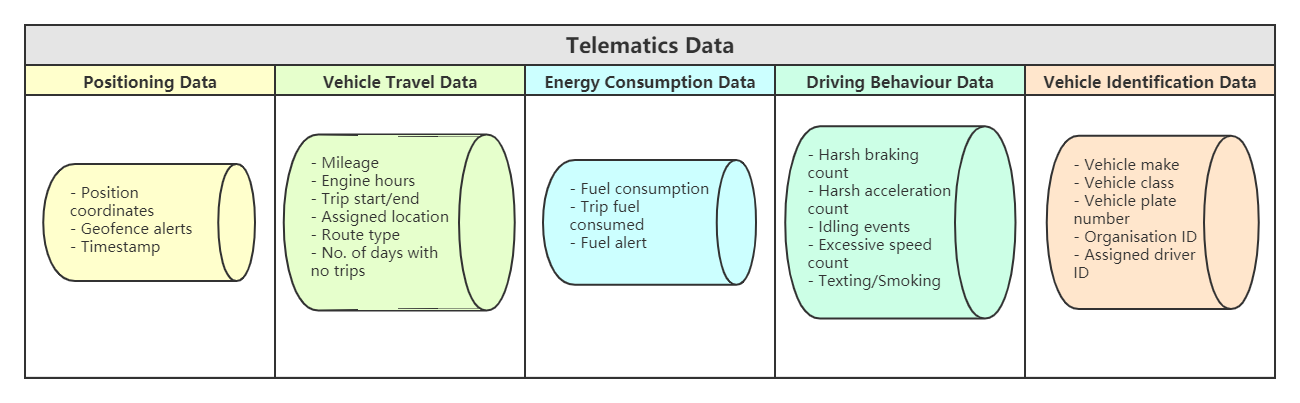
\includegraphics[width=\linewidth]{telematics category.png} %插入图片,[]中设置图片大小,{}中是图片文件名
\caption{Telematics data category (amended from \cite{RN160})} %最终文档中希望显示的图片标题
\label{fig1} %用于文内引用的标签
\end{figure}



\subsection{Step1: data selection and coordination}
\label{blockchain}

A complete set of telematics records for January 2015 to September 2015 was obtained from the fleet telematics company, which provides the service to our 40 tonne gross articulated HGVs used for supermarket deliveries. Each delivery vehicle is fitted with a telematics data transmitter that incorporates a GPS tracker and a link to the vehicle CAN bus which enables it to record data from a number of vehicle sensors with average resolution of 1 Hz. The data covers activities in the Greater London area and contains all deliveries from the depot to 42 London supermarkets. 

The raw telematics data was provided in two files. The first ‘Event’ file contained all the time-stamped, GPS records collected from each vehicle with time resolution of approximately five minutes. The second ‘Sensor’ file contained information from a number of sensors on the vehicles, such as cumulative distance, number of harsh accelerations and brakes applications, coasting time, and fuel consumption etc. The ‘Event’ and ‘Sensor’ files were linked to relate the sensor data to a location.  A unique identifier was available in the ‘Event’ file which corresponded to a specific tractor unit registration number and characteristics, such as make, model and EURO standard. 

With redundant sensor data available, it is paramount to select most relevant variables to the study. Based on the examination of data quality of each variable (percentage of NA value, extreme value feasibility etc.), 20 sensor variables are chosen for further data analysis. During basic data manipulation, units of each variable were confirmed, and the conversion between cumulative and discrete data were conducted. Coordinate system was picked according to the country being investigated and the software tools being used.


\subsection{Step2: route identification}
\label{blockchain}
\subsubsection{OD pairs and trips with direction development}
\label{insurance}

One of the key step of applying discrete truck GPS data is to link them with real-life delivery trips with directions. Following the steps in Figure 2, individual trips with the direction of travel are developed. First, vehicle movements were separated by operating time of day (that is, LLCS or non-LLCS hours). Then vehicle GPS records were clustered according to the concept of “Geo-fencing”, either near the depot (DC) or close to the supermarkets (store). At last, given an origin (or destination), a threshold of time interval per trip was set, within which the paired destination (or origin), based on the adjacent arrival (or departure) timestamp, was traced. More details are in the logic graph in Appendix B.

\subsubsection{Multi-drops and detour detection}
\label{insurance}
Non-typical movements, such as detours, multi-drops, and other route variability, were excluded from the analysis.  As is in Figure 2, for trips during LLCS hours, trip lengths was compared with the distance of LLCS routes defined using the company’s route planning GIS shapefile; while for trips during non-LLCS time, the shortest route length was chosen as the benchmark for comparison. Those trip length discrepancy greater than the threshold proposed (say 3km) were detected as detours, multi-drops or other route variability. Although the method seems too simple, it is verified that 90$\%$ of trips occurred along the LLCS routes during the overnight period when the noise restrictions were in force; and 85$\%$ of the non-LLCS routes occurred during the daytime period when noise restrictions were lifted. More details are in the logic graph in Appendix B. 

\subsection{Step3: Impacts quantification and visualization}
\label{blockchain}

Given the identified trips in previous step, the sensor data corresponding to each of them is then joined together with their GPS records. More specifically, each trip is characterized by information about speed, driving time, journey distance, number of accelerations, brake applications, fuel consumption etc. during a certain time period on a series of geographic points denoted by their GPS records. Then, the impacts of policy in terms of changes in traveled route lengths, vehicle speed, overall driving time, fuel consumption and fuel efficiency etc., in and out of the policy restriction time period, can be quantified and visualized using R software. The analysis can be conducted on two facets: one is at the aggregate level viewing the overall changes of the mentioned variables on the entire affected geographical area; and the other is at the local level, for example showing changes of vehicle operations on specific routes within shorter period of time. Moreover, the spatio-temporal distribution of those changes can be visualized on map through tableau software.



\begin{figure}[H] %H为当前位置,!htb为忽略美学标准,htbp为浮动图形
\centering %图片居中
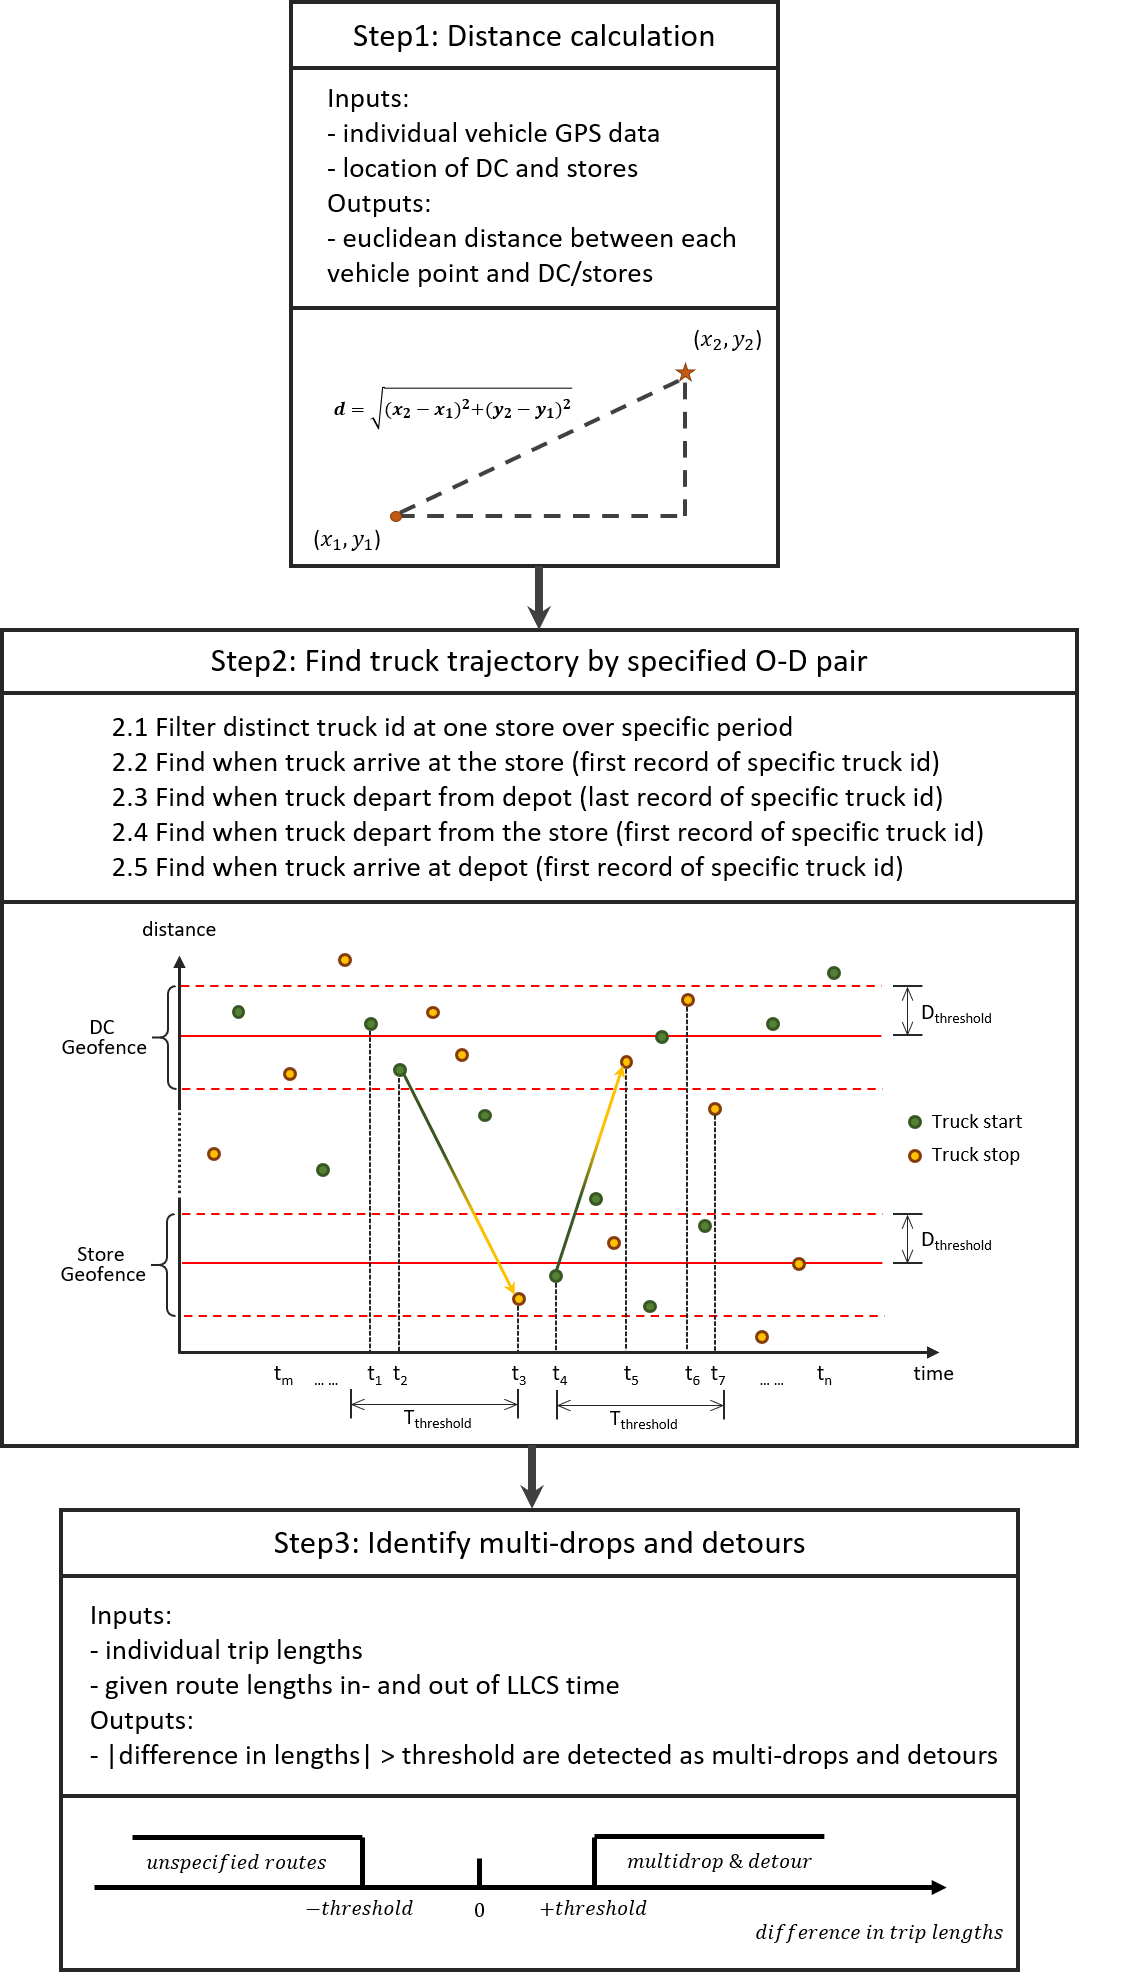
\includegraphics[scale=0.7]{figure2.png} %插入图片,[]中设置图片大小,{}中是图片文件名
\caption{Methodology for identifying OD pair} %最终文档中希望显示的图片标题
\label{fig2} %用于文内引用的标签
\end{figure}




\section{Results and discussion}
\label{sec4}


\subsection{Changes in vehicle operations in and out of LLCS control period on a general scale}

This study takes one-month data (June 2015) as a case example to apply the proposed methodology. In June, there were in total 4,211 deliveries (56.7$\%$ of overall deliveries) during LLCS hours and 3,213 deliveries (43.3$\%$ of overall deliveries) during non-LLCS hours. Total vehicle distance traveled during the study period (June 2015) was 210,068.38 km, and the vehicle fleet consumed a total of 66,212.01 liters of diesel. As is calculated from Table 4, 60.20$\%$ of distance traveled and 59.52$\%$ of fuel consumed are in LLCS hours, which are all larger than the percentage of number of deliveries (56.7$\%$) in LLCS hours. Thus it is hypothesized that the LLCS restrictions on routes leads to additional vehicle mileage and fuel consumption at the aggregate level. This can be justified by data from Table 5, which shows the mean and standard deviation value of trip distance and trip fuel consumption. 


\begin{table}[H]
\footnotesize
\centering
\caption{Summary of total vehicle distance traveled and fuel consumption in June during different time period}
\label{tbl4}
\begin{tabular}{m{3cm}<{\centering} m{3cm}<{\centering} m{4cm}<{\centering}}
\toprule[1.2pt]
  \textbf{Time period} &\textbf{Total distance traveled (km)} &\textbf{Total fuel consumption (liter)} \\


  \midrule
   LLCS & 126,466.70 & 39,412.43  \\
   
   nonLLCS & 83,601.68 & 26,799.58  \\
   

   overall & 210,068.38 & 66,212.01 \\

  \bottomrule[1.2pt]
  \end{tabular}
\end{table}


As for other data in Table 5, the trip distance deviation in LLCS hours is smaller than that in non-LLCS hours, in other words, given that each route has fixed length, the route choice in non-LLCS time period has a relatively higher variety. From Figure 3, it is logical to see less average fuel consumption in non-LLCS hours, since, on average, vehicles were operating on shorter routes for individual trip with similar fuel efficiency level in non-LLCS hours. However, the average standard deviation of fuel efficiency per trip in non-LLCS hours is higher than that in LLCS hours, which means that the fuel efficiency benefit in non-LLCS hours is not applicable to all trips. Considering many factors could affect fuel efficiency level of a trip, for example, aggressive driving, excessive idling, higher speed, excessive cargo weight, cold weather and hilly terrain or unpaved roads can all reduce fuel economy. The available data is not sufficient to explain the reason for differences in fuel efficiency in different time period on an aggregate level. Thus, more detailed investigation on specific routes were conducted, and relevant results will be discussed in next section.


\begin{table}[H]
\footnotesize
\centering
\caption{Summary of mean and standard deviation value of average vehicle distance traveled, average fuel consumption and average fuel efficiency per trip in June during different time period}
\label{tbl5}
\begin{tabular}{ccccccc}

\toprule[1.2pt]
  \multirow{2}{*}{\textbf{\shortstack{Time \\period}}} & 
  \multicolumn{2}{c}{\textbf{\shortstack{Distance traveled\\ per trip (km)}}} &
  \multicolumn{2}{c}{\textbf{\shortstack{Fuel consumption\\ per trip (liter)}}} &
  \multicolumn{2}{c}{\textbf{\shortstack{Fuel efficiency \\per trip (km/liter)}}}\\
  
  \specialrule{0em}{2pt}{1pt}
 
  
  & mean & \shortstack{standard\\ deviation} & mean & \shortstack{standard\\ deviation}& mean & \shortstack{standard\\ deviation} \\ 
    
  \midrule
   LLCS & 30.03 & 13.56 & 9.36 & 4.73 & 3.32 & 0.72 \\
   
   nonLLCS & 26.02 & 14.14 & 8.34 & 4.86 & 3.33 & 0.83  \\
   
  \bottomrule[1.2pt]
  \end{tabular}
\end{table}


\begin{figure}[H] %H为当前位置,!htb为忽略美学标准,htbp为浮动图形
\centering %图片居中
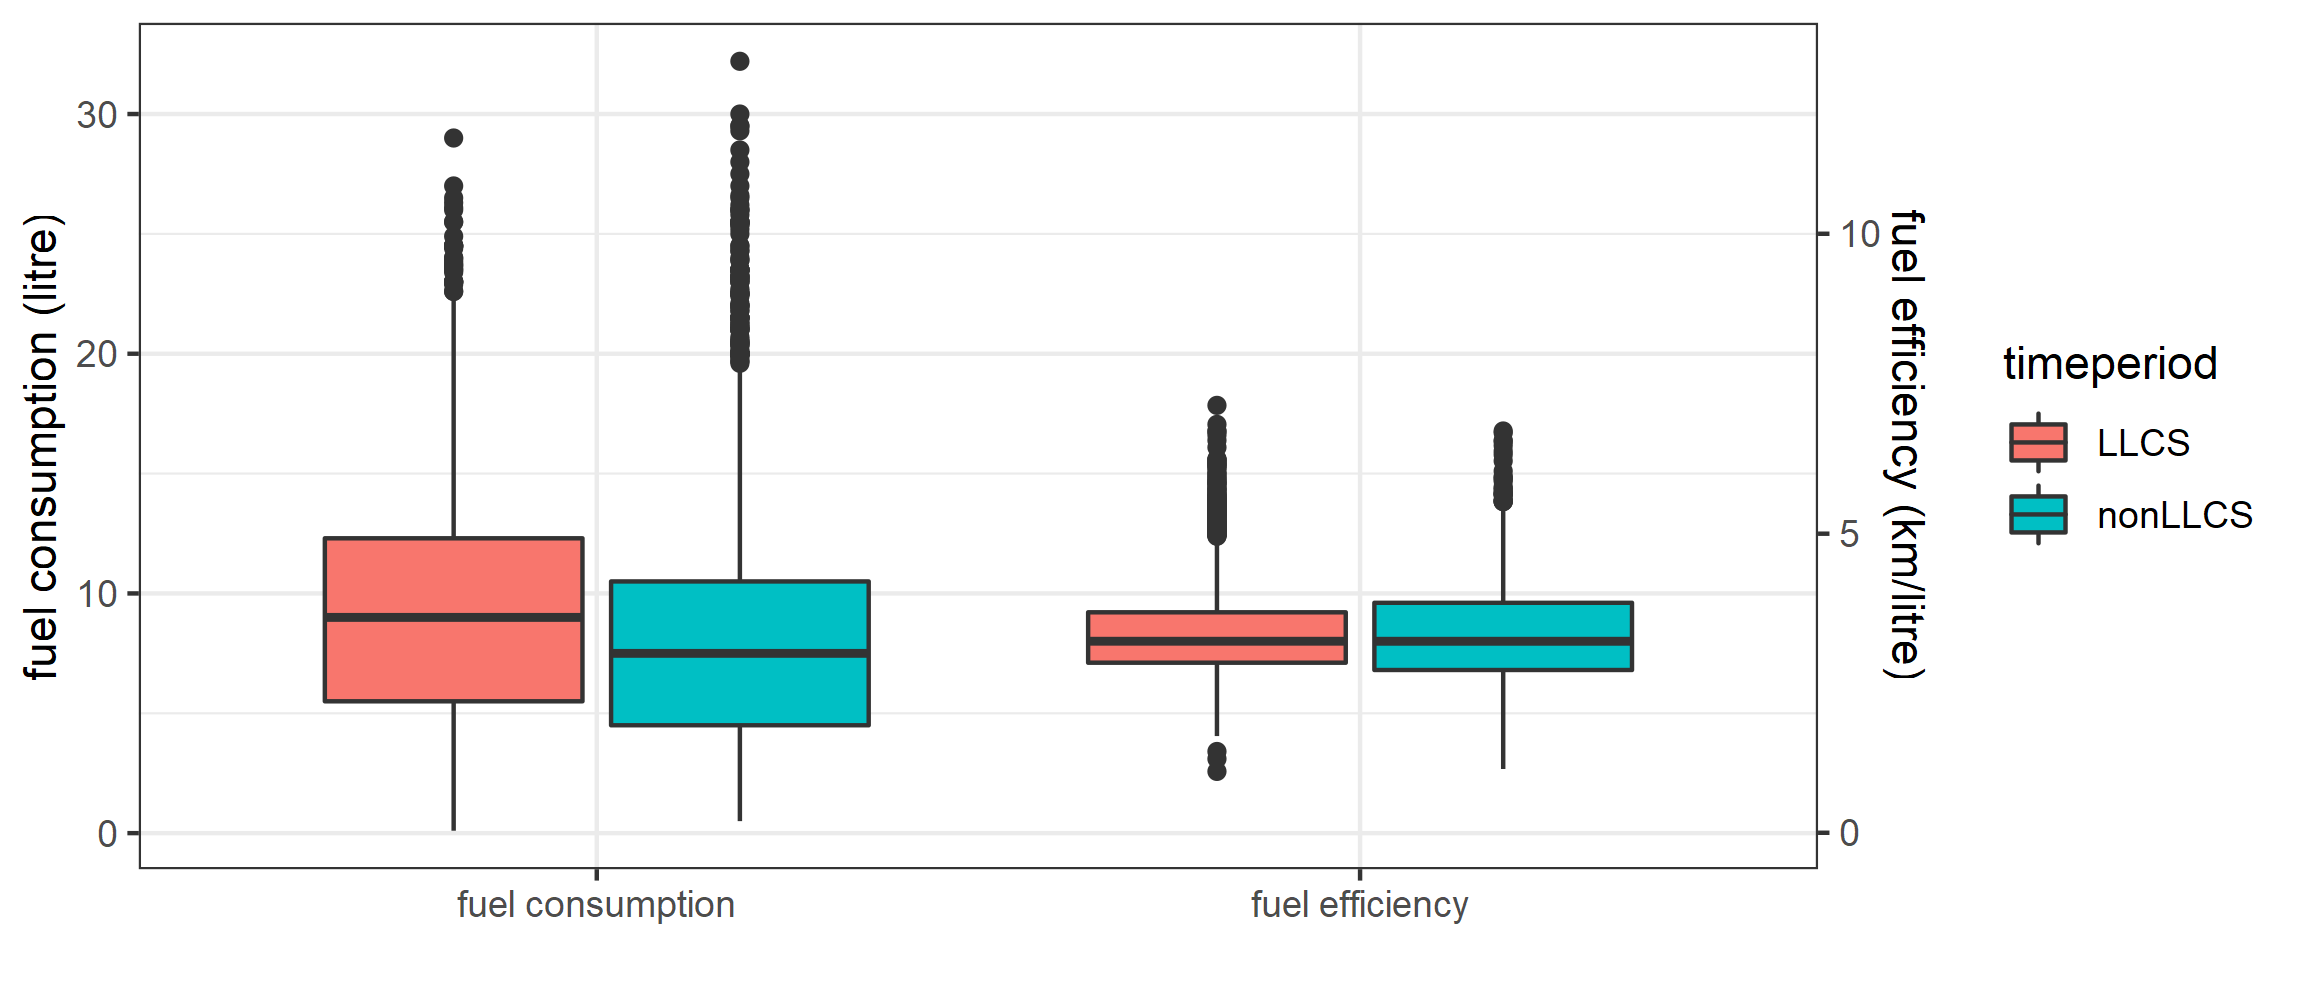
\includegraphics[scale=0.8]{fuelrelated.png} %插入图片,[]中设置图片大小,{}中是图片文件名
\caption{boxplots of average fuel consumption and fuel efficiency per trip during LLCS and non-LLCS hours in June} %最终文档中希望显示的图片标题
\label{fig3}
\end{figure}



In addition to analyzing the outcome of a trip (e.g. distance traveled and fuel consumed), the in-process attributes of it (e.g. level of congestion, driver operation) are studied as well. In terms of the driving condition (in the sense of level of congestion), it can be figured out from Figure 4 that, at an aggregate level, the average trip speed is higher during LLCS hours, and is with larger variety during non-LLCS hours. Due to the characteristics of vehicle speed on road, although trip distance is relatively longer in LLCS hours, the mean value of the average trip duration are similar during different time period (LLCS and non-LLCS hours), and the variation of trip duration is less stable in non-LLCS hours. 

These are reasonable, in that the LLCS hours are during night time when traffic volumes are lower than that in non-LLCS hours (during day time); and the HGVs are restricted to the ERN which comprises major roads with higher speed limits. Furthermore, vehicles may come across more uncertainties on road during day time (non-LLCS hours), which leads to the situation that shorter routes may even take longer time in non-LLCS hours. The records indicating driving behavior (i.e. harsh acceleration and break application per trip in Table 6) could support this statement, that on average extra number of breaks and harsh accelerations per trip are identified in non-LLCS hours.



\begin{figure}[H] %H为当前位置,!htb为忽略美学标准,htbp为浮动图形
\centering %图片居中
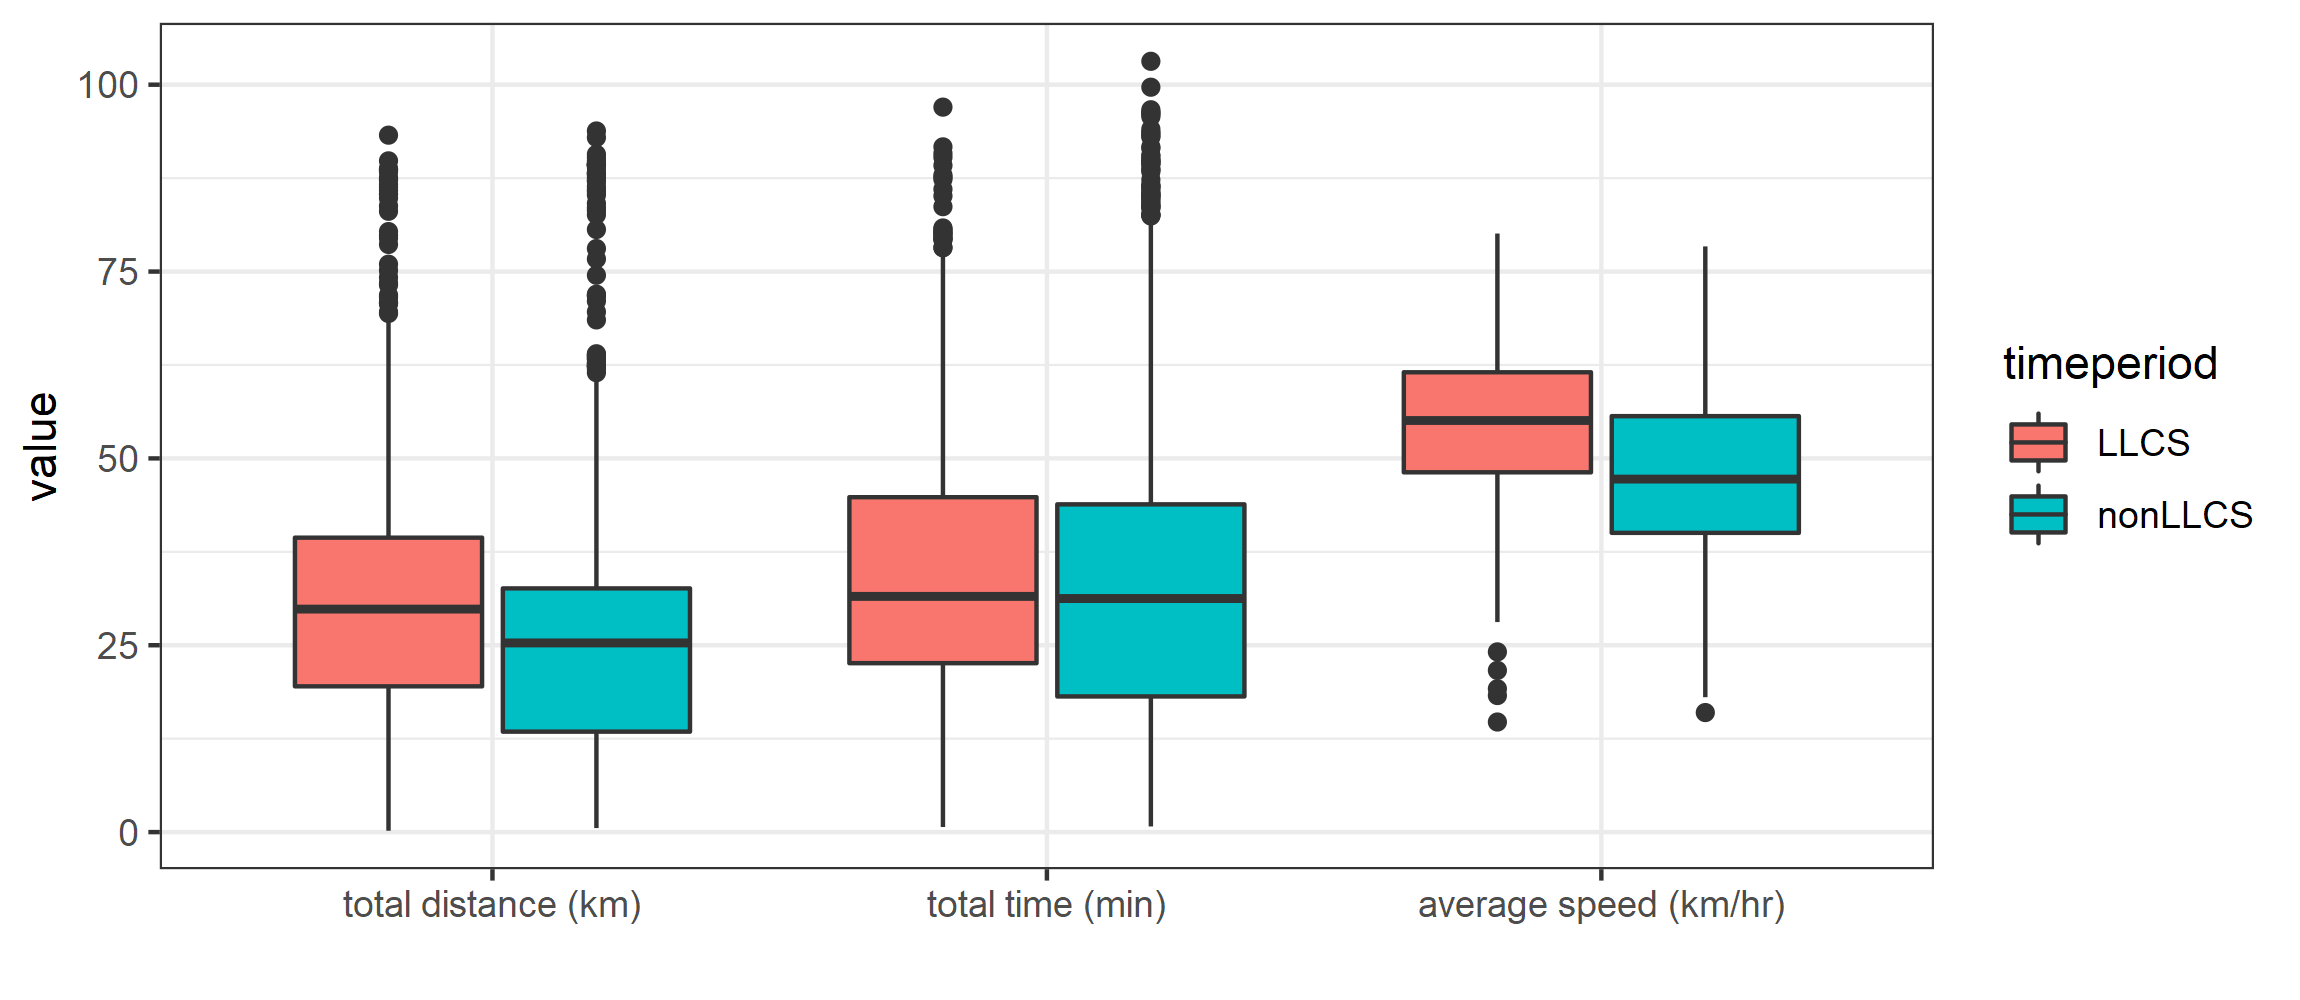
\includegraphics[scale=0.8]{ dist_time_speed.png} %插入图片,[]中设置图片大小,{}中是图片文件名
\caption{boxplots of average distance traveled, average driving time, and average speed per trip during LLCS and non-LLCS hours in June} %最终文档中希望显示的图片标题
\label{fig4} %用于文内引用的标签
\end{figure}



\begin{table}[H]
\footnotesize
\centering
\caption{Summary of mean and standard deviation value of average number of break application and harsh acceleration per trip in June during different time period}
\label{tbl6}
\begin{tabular}{ccccc}

\toprule[1.2pt]
  \multirow{2}{*}{\textbf{\shortstack{Time \\period}}} & 
  \multicolumn{2}{c}{\textbf{\shortstack{Break application\\ per trip}}} &
  \multicolumn{2}{c}{\textbf{\shortstack{Harsh acceleration \\per trip}}}\\
  
  \specialrule{0em}{2pt}{1pt}
 
  
  & mean & \shortstack{standard\\ deviation} & mean & \shortstack{standard\\ deviation}\\ 
    
  \midrule
   LLCS & 50.74 & 8051.91  & 3.00 & 4.65 \\
   
   nonLLCS & 97.85 & 7432.20 & 4.09 & 5.45 \\
   
  \bottomrule[1.2pt]
  \end{tabular}
\end{table}


After pure data manipulation and relationship exploration, for better understanding the spatio-temporal distribution of above variables that has been investigated, maps demonstrating the speed and fuel economy attributes of trips during LLCS and non-LLCS hours are depicted in Figure 5 and Figure 6, respectively.

In Figure 5, darker green grids indicate higher speed in km/hr, while lighter green grids denote that vehicles traveled slower in those area. As is given previously that overall average speed was higher (54 km/hr) in LLCS hours than in non-LLCS hours (48 km/hr), the geographical feature of speed variation is revealed, that in general the speed of the vehicles fell 50$\%$ as they approached central London (defined as zones within congestion charging area) during both LLCS and non-LLCS hours. Also, Figure 5A shows vehicles used the longer route during LLCS hours and made detours to their destination stores (highlighted in the red circles a and b in Figure 5A). Figure 5B shows a larger number of routes during non-LLCS hours, especially inside the city (highlighted in the red circles c, d and e in Figure 5B). Also, there were no deliveries observed during LLCS hours for one supermarket near Harrow (See Figure 5, the red circle f). 

Figure 6A and B illustrate the spatio distribution (0.5 x 0.5 km grid) of fuel economy (liter/100 km) reported by the vehicle telematics. Fuel economy is about 13$\%$ better in LLCS hours (31 liter/100 km) than non-LLCS hours (35 liter/100 km); besides, the distribution of fuel economy is quite similar to that of vehicles speeds in Figure 5A and B, implying the positive relationship between speed and fuel economy.




\begin{figure}[h]          
    \mbox{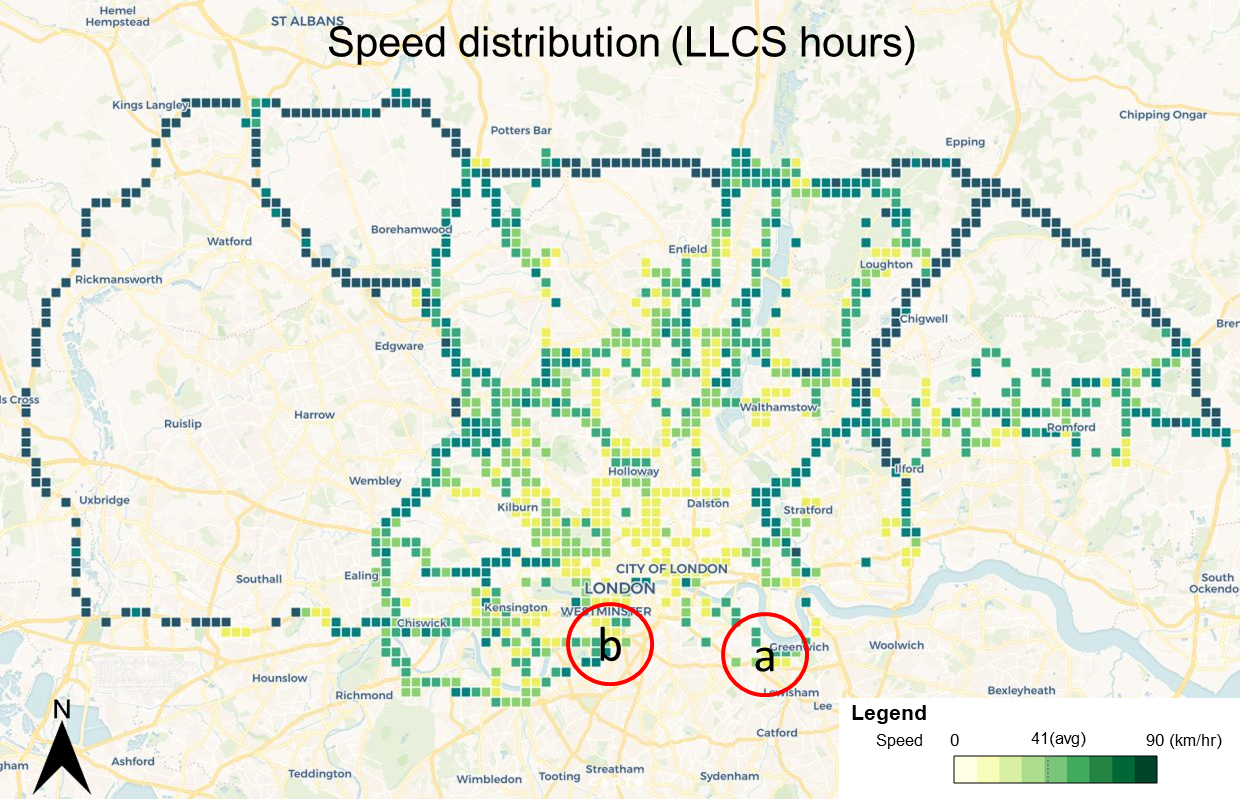
\includegraphics[scale=0.78]{llcsspeed.png}}   
    \hspace{0.1px}
    \mbox{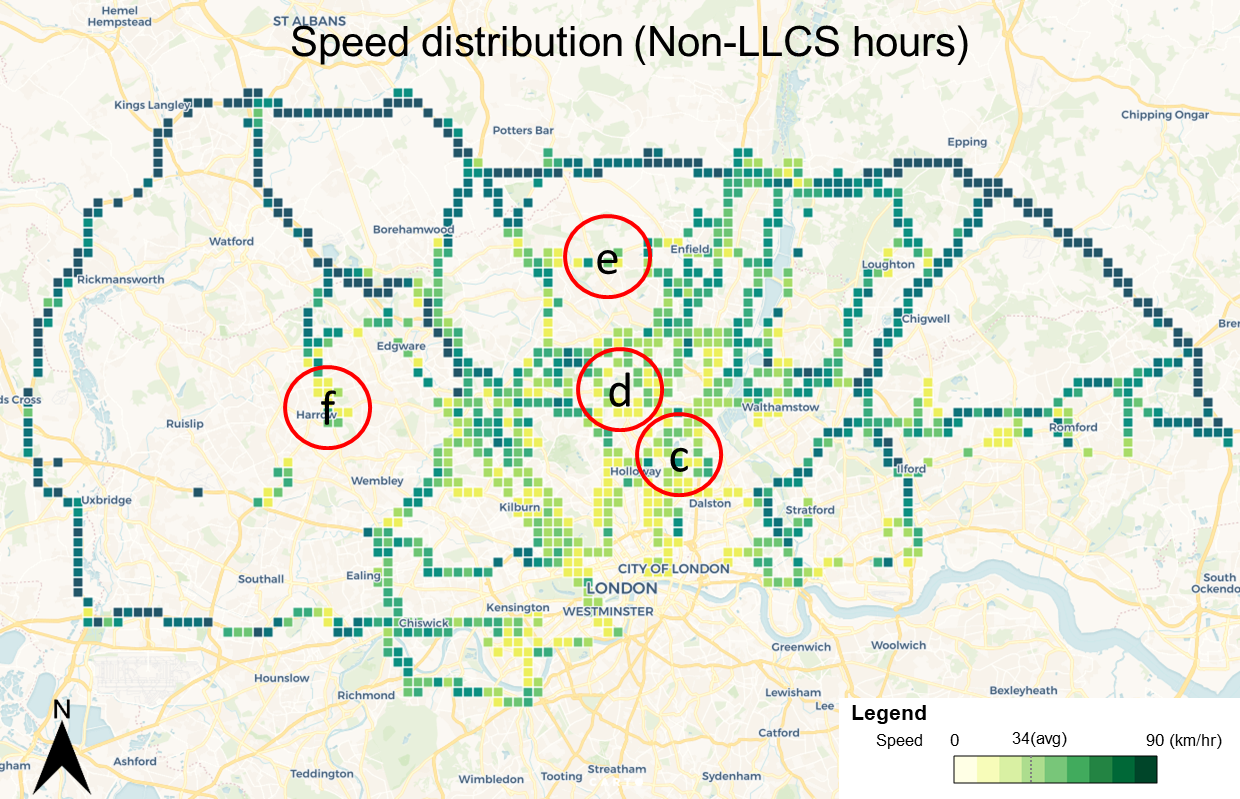
\includegraphics[scale=0.78]{nonllcsspeed.png}}
    \caption{left: A: Speed distribution (km/hr) during LLCS hours in June; right: B: Speed distribution (km/hr) during non-LLCS hours in June}
    \label{fig5}
\end{figure}



\begin{figure}[h]          
    \mbox{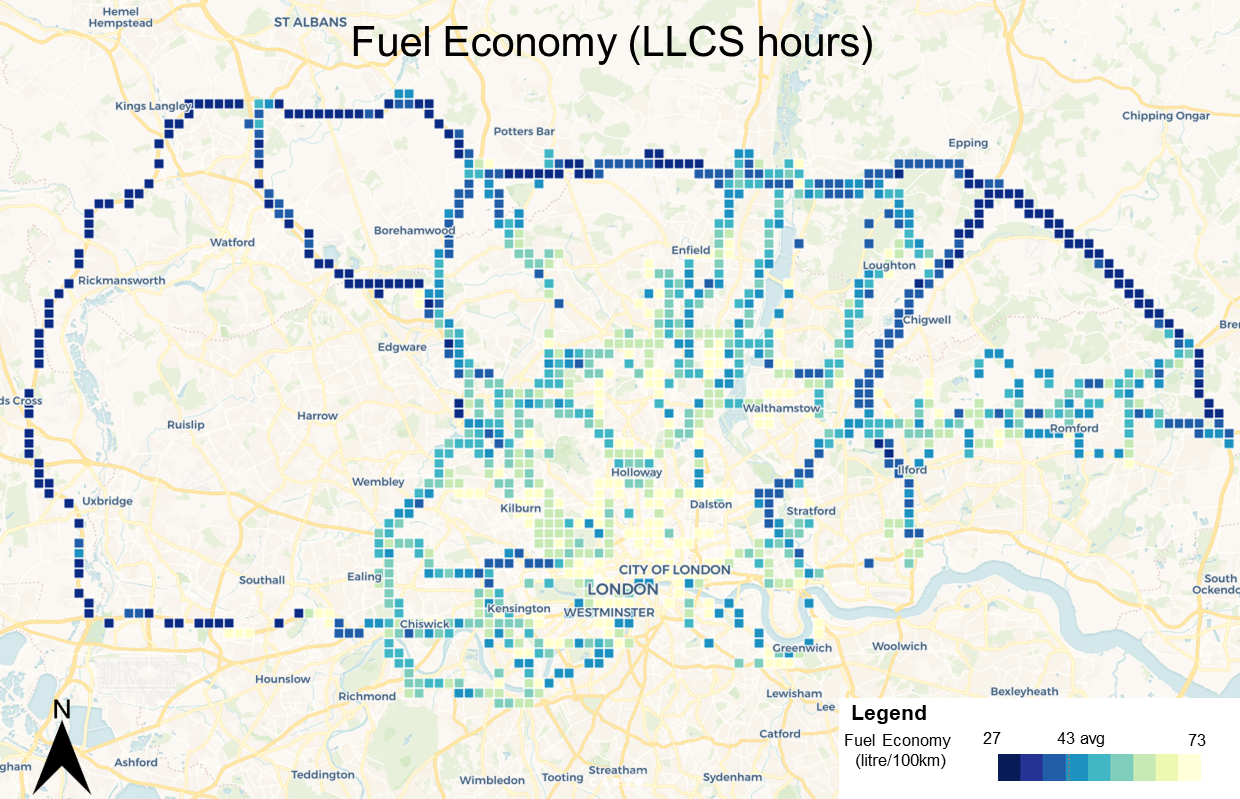
\includegraphics[scale=0.78]{llcsfuel.png}}   
    \hspace{0.1px}
    \mbox{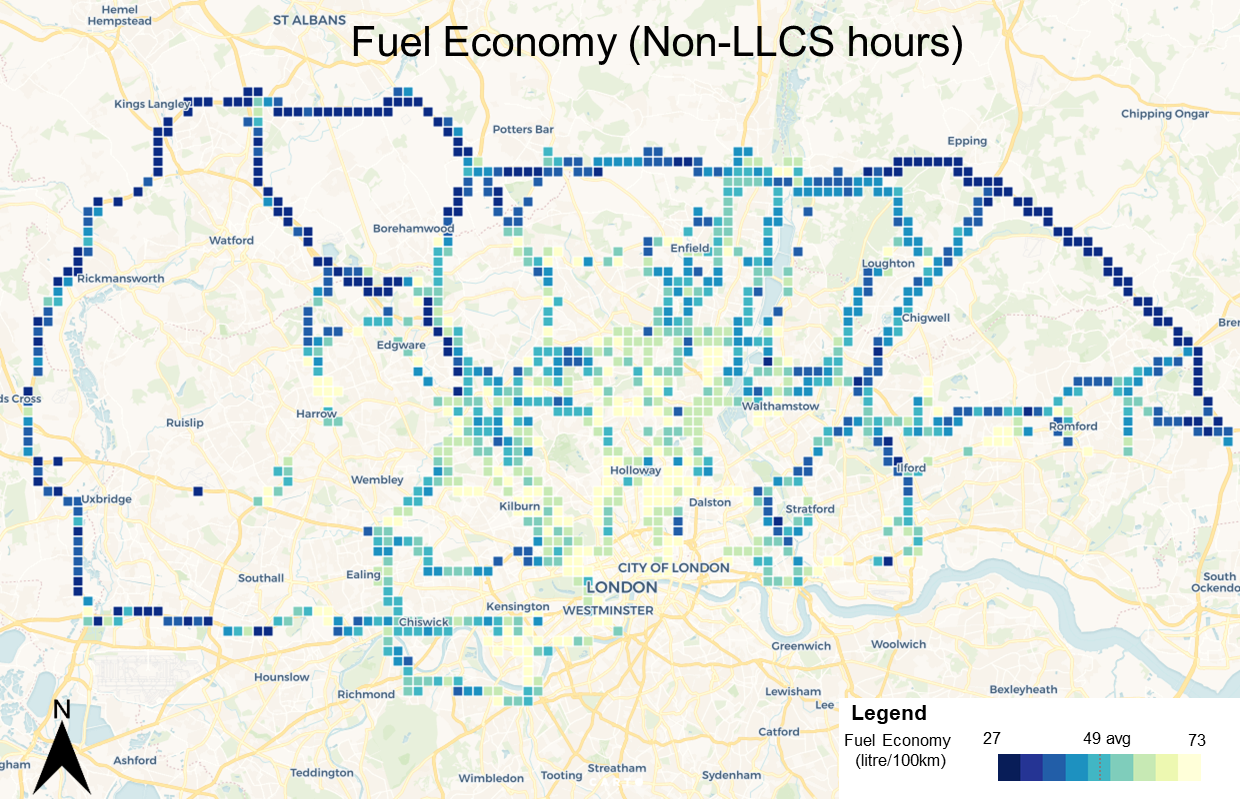
\includegraphics[scale=0.78]{nonllcsfuel.png}}
    \caption{left: A: Fuel economy (liter/100km) during LLCS hours in June; right: B: Fuel economy (liter/100km) during non-LLCS hours in June}
    \label{fig6}
\end{figure}





\subsection{Detailed investigation on specific routes of changes in vehicle operations in and out of LLCS control period }

To carry on with the discussions in previous section about the differences in fuel economy during different time period, specific origin-destination pairs (OD pairs) are selected based on their trip characteristics for detailed investigation. More specifically, first, for the purpose of higher data availability in both time period, the frequency of trip traveled for each OD pair is displayed in Figure 7. Those OD pairs which either have comparable trip frequency value during different time period (LLCS hours and non-LLCS hours) or have relatively higher trip frequency value themselves, are selected (showed in Table 7).




\begin{figure}[H] %H为当前位置,!htb为忽略美学标准,htbp为浮动图形
\centering %图片居中

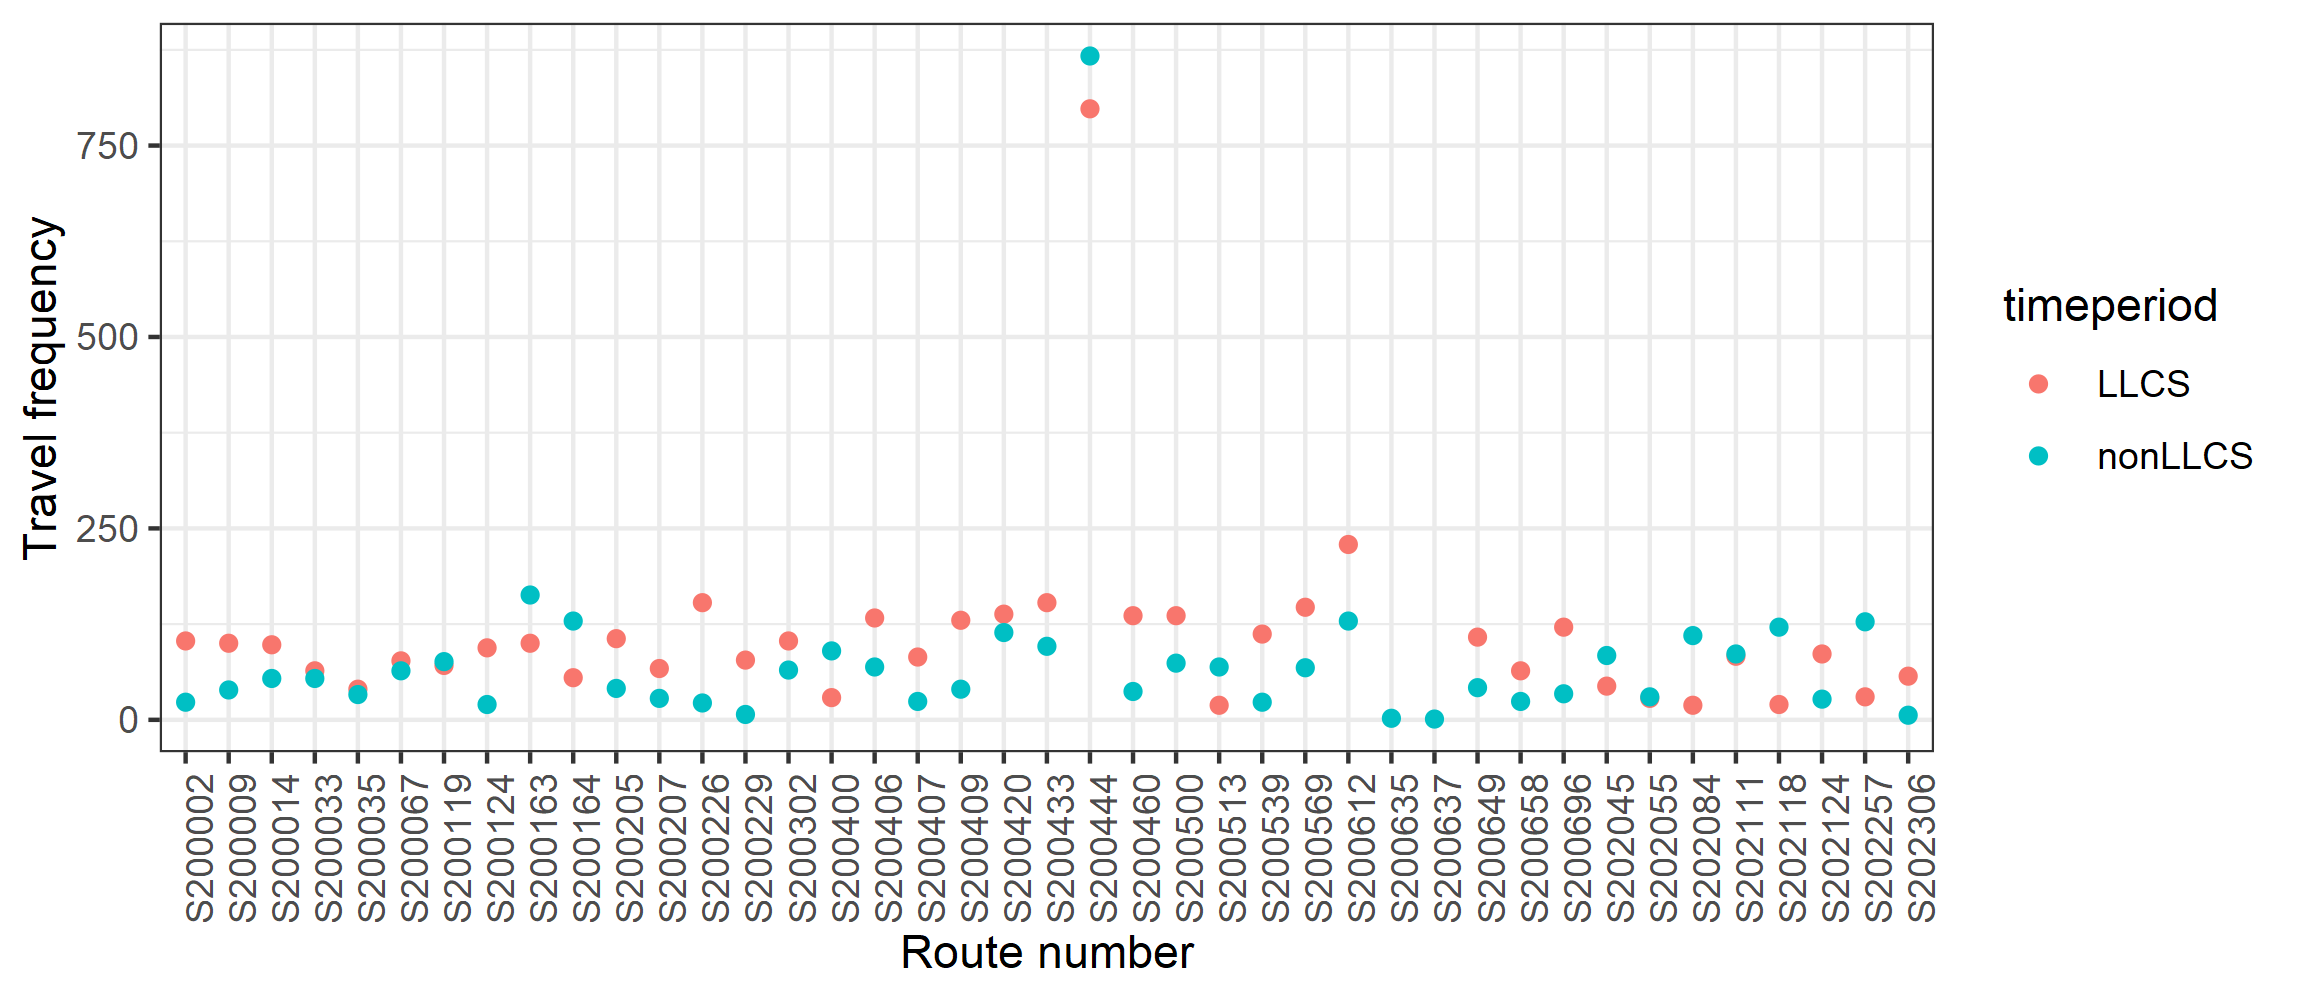
\includegraphics[scale=0.9]{routefreq.png} %插入图片,[]中设置图片大小,{}中是图片文件名
\caption{scatter plot for trip frequency on each OD pair denoted by route number during different time period} %最终文档中希望显示的图片标题
\label{fig7}
\end{figure}




\begin{table}[H]
\footnotesize
\centering
\caption{trip frequency information on selected OD pair (noted by route number)}
\label{tbl7}
\begin{tabular}{m{2cm}<{\centering} m{4cm}<{\centering} m{4cm}<{\centering} m{3cm}<{\centering}}
\toprule[1.2pt]
  \textbf{Route number} &\textbf{Trip frequency in LLCS hours} &\textbf{Trip frequency in nonLLCS hours} &\textbf{Difference in trip frequency} \\


  \midrule
   S202111 & 83 & 86 & -3\\
   S200119 & 71 & 76 & -5\\
   S200067 & 77 & 64 & 13\\
   S200420 & 138 & 114 & 24\\
   S200302 & 103 & 65 & 38\\
   S200163 & 100 & 163 & -63\\
   S200444 & 798 & 867 & -69\\
   S200612 & 229 & 129 & 100\\
   
  \bottomrule[1.2pt]
  \end{tabular}
\end{table}

Then, for each OD pair, a scatter plot showing the relationship between trip driving time and trip fuel consumption is drew in Figure 8. It is found that with the exception of the top-left sub-figure (S200067), which contains relatively small amount of data points and are mostly overlapping on each other, the driving time variation for the same OD pair in both LLCS and non-LLCS hours is 10-20 mins. Besides, generally speaking, except for S200119, the trip driving time in non-LLCS hours is longer than that in LLCS hours, suggested by a slight rightward shift from orange to blue cluster in every sub-figure. 

Moreover, three sub-figures (S200119, S200444, and S200612) present a positive relationship between trip fuel consumption and trip driving time; while in other sub-figures, the trip fuel consumption value is invariant or maintains within a small range across different trip driving time. When comparing with the corresponding sub-figure according to route number in Figure 9, their point distribution pattern varies: the similar positive relationship between trip fuel consumption and trip distance traveled is found to exist in all sub-figures. With above observations, it is speculated that the increasing driving time in non-LLCS hours is not solely related to increasing distance traveled. In more detail, taking the sub-figure in the middle of Figure 9 (S200420) as an example, the variation in trip distance in non-LLCS hours is quite small; the value of trip lengths for that OD pair are converged to 20 km. However, with comparable trip lengths, the time needed to finish the trip varies from 20 mins to 40 mins. By way of explanation, for the OD pair noted by S200420, speed changes across trips; and is relatively lower in non-LLCS hours.


\begin{figure}[H] %H为当前位置,!htb为忽略美学标准,htbp为浮动图形
\centering %图片居中

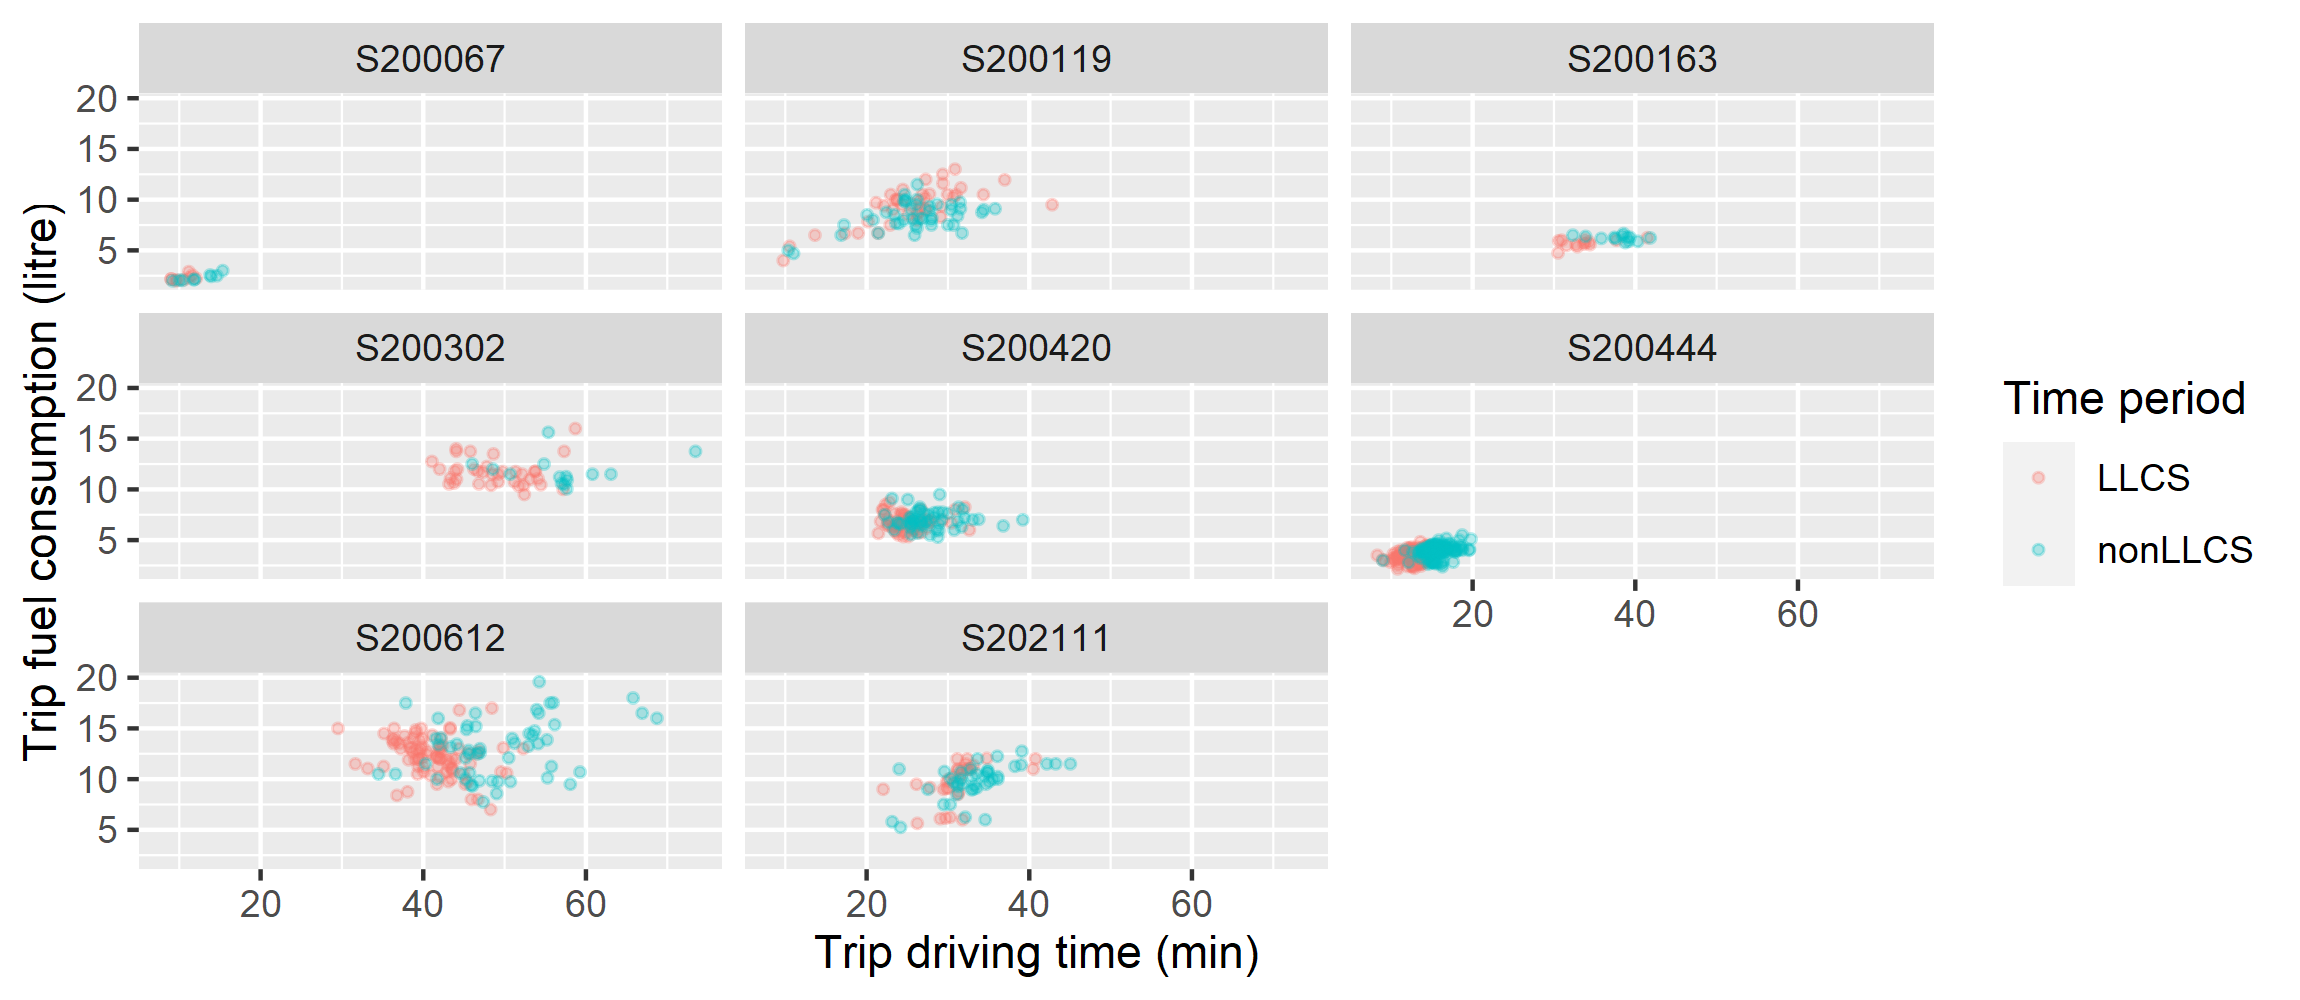
\includegraphics[scale=0.9]{selecteroute_time_fuel.png} %插入图片,[]中设置图片大小,{}中是图片文件名
\caption{scatter plot of trip driving time versus trip fuel consumption on specific OD pair during different time period in June (caption for each sub-figure is route number)} 
\label{fig8}
\end{figure}



\begin{figure}[H] %H为当前位置,!htb为忽略美学标准,htbp为浮动图形
\centering %图片居中

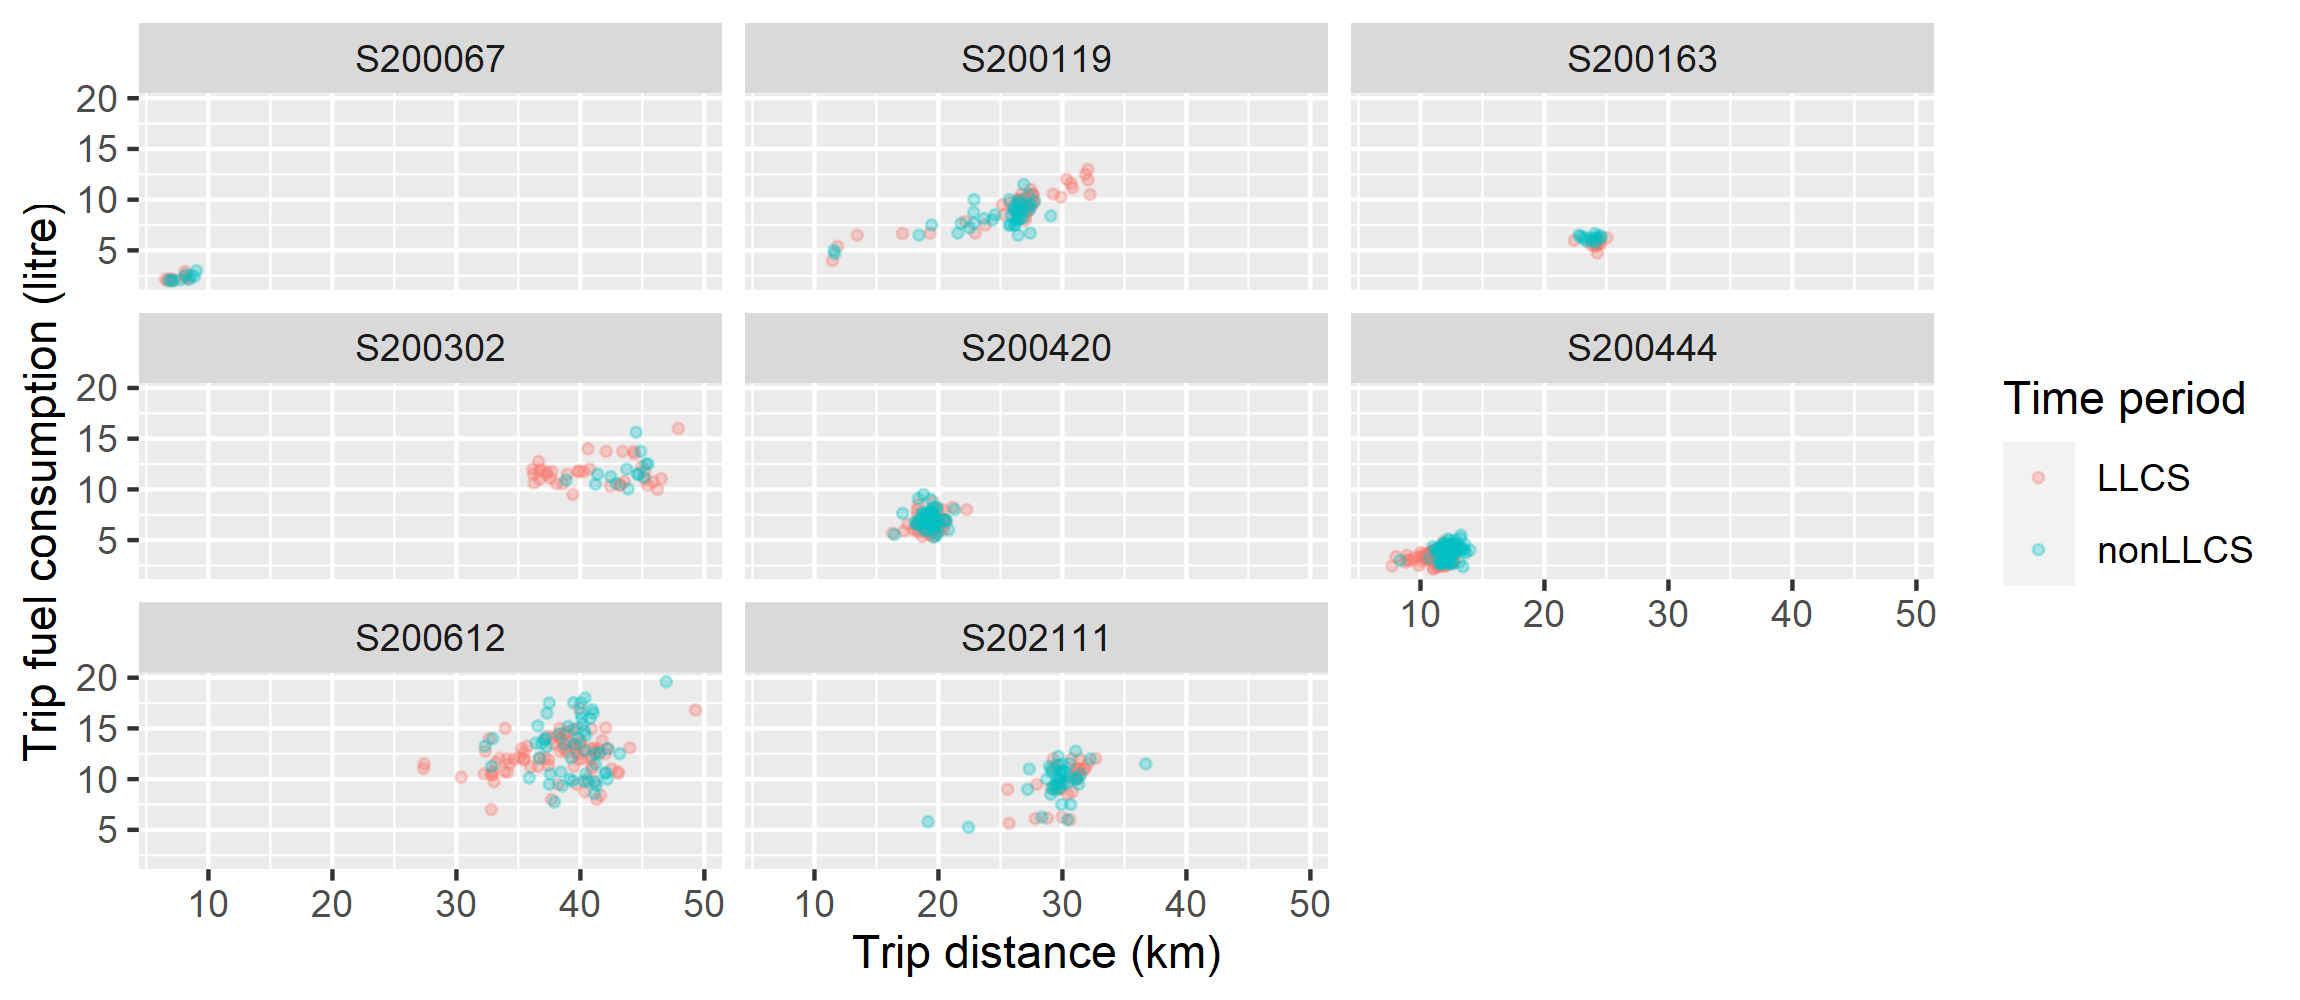
\includegraphics[scale=0.9]{selecteroute_dist_fuel.png} %插入图片,[]中设置图片大小,{}中是图片文件名
\caption{scatter plot of trip distance versus trip fuel consumption on specific OD pair during different time period in June (caption for each sub-figure is route number)} 
\label{fig9}
\end{figure}


Since trip fuel consumption (liter) is the multiplication of distance (km) and fuel efficiency (liter/km), and speed plays an important role in affecting both elements, data exploration on speed was carried out. Besides, considering that among those variables which could influence fuel efficiency level, only the number of harsh accelerations per trip variable has sufficient data availability in the dataset, it is analyzed together with speed. For a more clear demonstration, one OD pair with contrasting points distribution pattern during LLCS and non-LLCS hours in Figure 8 and 9 is chosen (S200444), and the results with respect to the relationship between fuel efficiency and speed and number of harsh accelerations are showed in Figure 10. 


\begin{figure}[H] %H为当前位置,!htb为忽略美学标准,htbp为浮动图形
\centering %图片居中

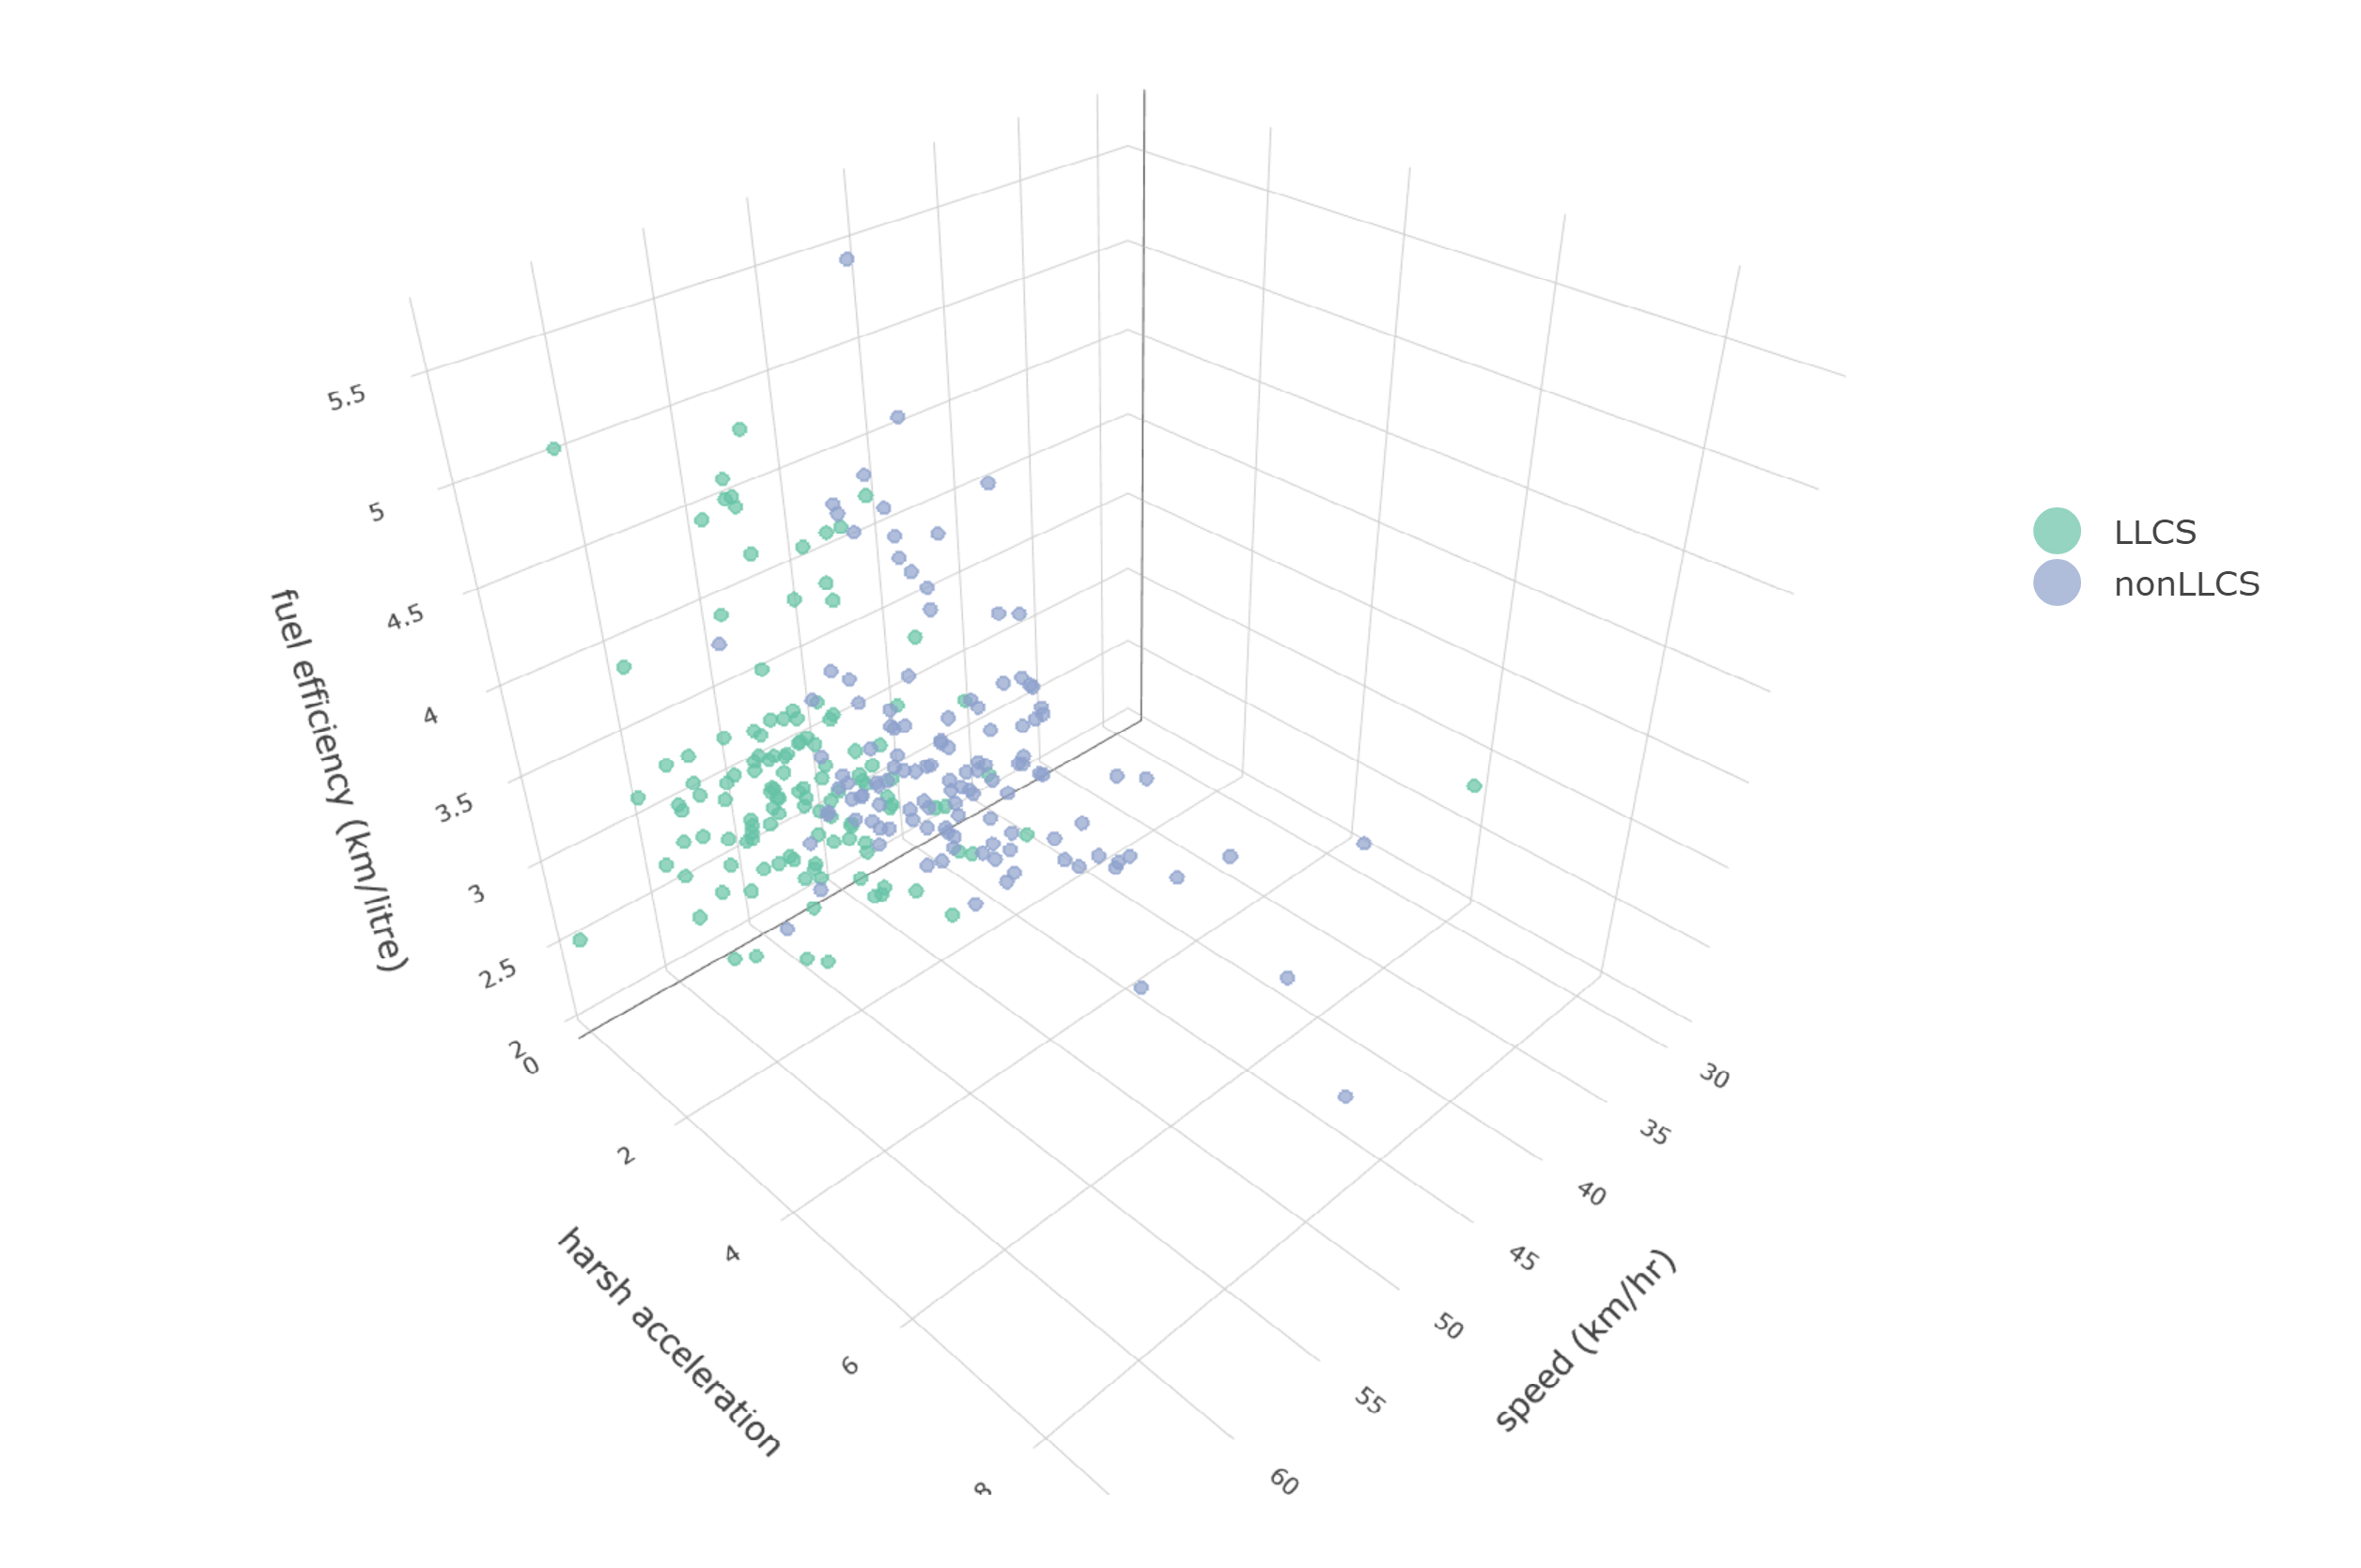
\includegraphics[width=1.0\textwidth]{3d_vafe.png} %插入图片,[]中设置图片大小,{}中是图片文件名
\caption{3D scatter plot of relationship among trip speed, number of harsh acceleration, and trip fuel efficiency on specific OD pair (route S200444) during different time period in June} 
\label{fig10}
\end{figure}

The specific trip has higher overall fuel efficiency level during LLCS hours, indicated by the upward location of the green points cluster. In terms of the reasons for it, from the 3D graph in Figure 10, in LLCS hours, despite of the outliers, drivers tend to apply harsh accelerations less often and employ higher vehicle speed (ranging from 45 to 65 km/hr). In contrast, during non-LLCS hours, trips are limited to a lower speed range of 30-55 km/hr, and more harsh acceleration are found. 

These results are further justified by the real-life driving conditions on that specific OD pair. According to the telematics data, for this OD pair, the roads traveled by trucks are the same in different time period; but one section of the road is quite likely to be congested in non-LLCS hours (daytime), which impairs vehicle speed to a great extent; while the higher speed limit during LLCS hours and fewer traffic during night time result in higher vehicle speed, contradictorily. As for the higher number of harsh acceleration, it is guessed that more complex driving environment on roads induces more aggressive driving behavior; and drivers making deliveries during night time period may be more used to smooth driving which requires less physical movements, for perhaps safety and tiredness reasons. These findings conform to the inference at the aggregate level on the entire delivery network. 



Furthermore, as for other conclusions made at aggregated level in earlier section that LLCS could lead to extra mileage, and route choices in non-LLCS hours are more diverse than expected, they can be proved on specific trip level as well. Taking the OD pair noted by S200420 as an example, it can be seen that, in Figure 11, the distribution of the lengths of trip is more disperse during non-LLCS hours than in LLCS hours. With further help of vehicle telematics data, it is identified that there are in total 4 different routes chosen by drivers in non-LLCS hours, including one scheme-controlled route designated in LLCS hours. It is actually surprising to see vehicles still travel on the scheme-controlled route when LLCS restrictions were not active, since it is longer than those not restricted by the scheme, which is less economic in terms of fuel consumption and time utilization. 



\begin{figure}[H] %H为当前位置,!htb为忽略美学标准,htbp为浮动图形
\centering %图片居中
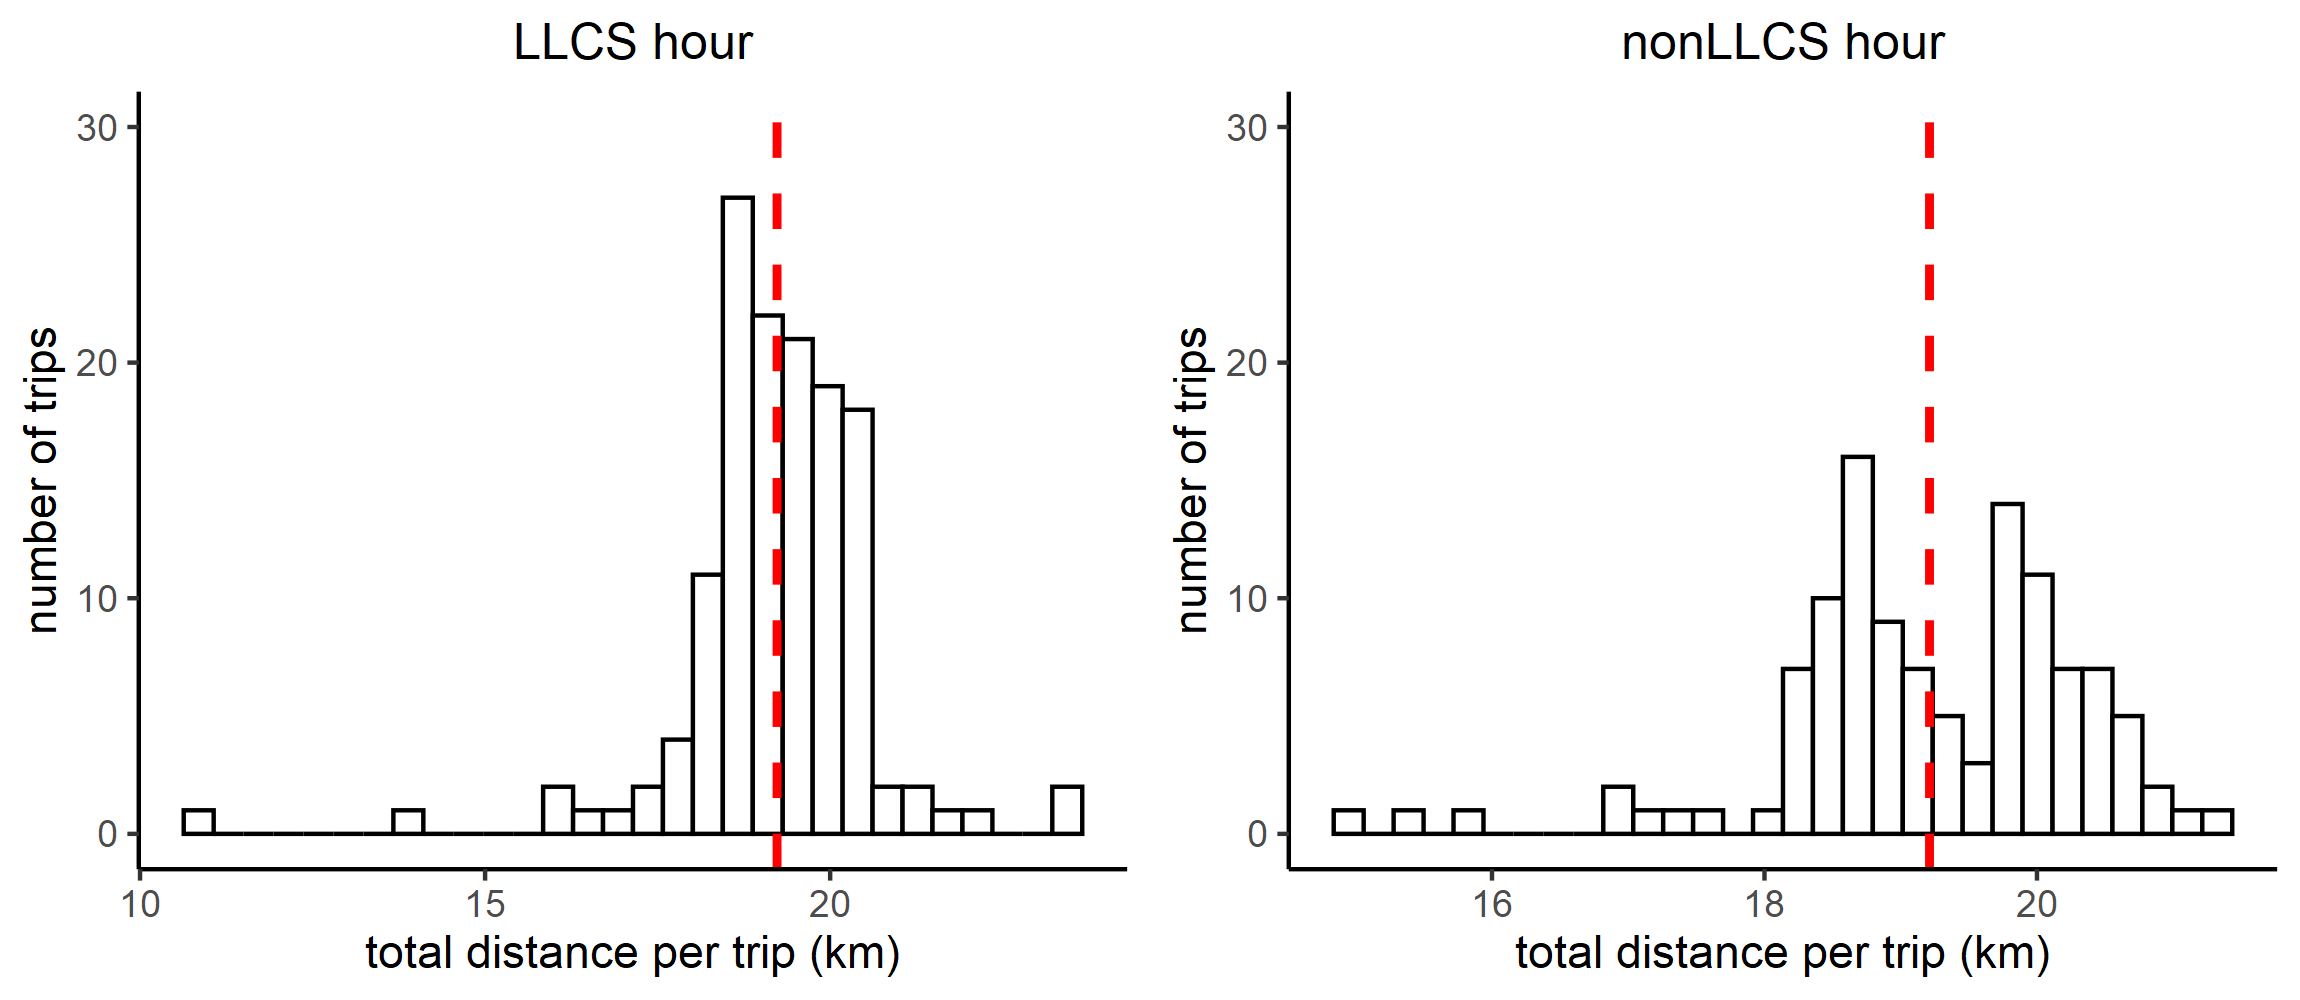
\includegraphics[scale=0.8]{S200420dist.png} %插入图片,[]中设置图片大小,{}中是图片文件名
\caption{distribution of total distance per trip on selected OD pair (S200420) during LLCS and non-LLCS hours in June (red line indicates mean value)} %最终文档中希望显示的图片标题
\label{fig11}
\end{figure}

As an indication of the scale of this issue, without assigning journeys to specific LLCS or non-LLCS routes, a total 210,068 vehicle km are observed from the telematics during the study period, of which 83,602 km are during non-LLCS hours. In contrast, applying our filters for defined LLCS and non-LLCS routes, it is estimated that there should be a total of 197,000 vehicle km traveled during the study period, of which 67,000 km are during non-LLCS hours. Thus, this sub-optimal route choice leads to an additional 13,068 vehicle km (6$\%$) in the study period overall. During non-LLCS hours total distance traveled is 20$\%$ higher than would be the case if the designate routes were followed. As a result, it is crucial for operators to pay more attention on delivery route design and the issue of drivers' compliance towards route selection.



\section{Conclusions and recommendations}

This is the first study to provide a general framework which is essential for providing robust quantitative-based evidence for urban freight transport policy evaluation and other telematics applications. It quantifies the differences in vehicle distance traveled, fuel consumption, speed and number of acceleration in and out of the LLCS controlled hours with visualized evaluations. 

This work has considered one part of the operation of a large UK haulier. Whilst we have no independent data on other companies, the observations in this paper are only applicable to the analyzed company in specified time period. Findings are obtained on two facets: first, at aggregate level, LLCS restrictions on routes leads to additional vehicle mileage and fuel consumption for the analyzed company. The average vehicle driving speed is higher and more stable during LLCS hours than in non-LLCS hours; and a smoother driving behavior is found more often in LLCS time period. These are suggested to be the significant reasons for the fuel efficiency benefits (13$\%$ better in LLCS time).

Second, at trip level, in addition to the verification of above findings on the entire transport network, it is identified that route choice in non-LLCS hours has higher variety than in LLCS hours. Some of the drivers did not follow the designed routes, choosing to stick to the specified routes, which are longer, restricted by the LLCS even though the policy were not active. It is calculated that, during the study period, this sub-optimal route choice increased vehicle km by 6$\%$ overall and 20$\%$ during non-LLCS hours relative to the idealized routes. Taking into considerations of the discoveries on the negative features of driving environment in non-LLCS hours, such as more complex road conditions and more congestion, leading to lower fuel efficiency level, it is logical to see a higher overall fuel consumption result.

These same issues could potentially be encountered by other operators in London. Our results therefore indicate that an unintended consequence of the LLCS could be to increase route distances at all times of the day. This issue could be avoided using improved route planning and guidance systems that account for the LLCS restrictions dynamically. Moreover, more effort should be devoted to driver training with respect to route compliance and smooth driving, otherwise the issues of higher overall fuel consumption and longer delivery time would exist.


In conclusion, as for the case study of LLCS, a broader cost-benefit analysis is necessary, which involves other hauliers' operations data and incorporates noise, emissions, and social and economic impacts in a wider sense. More importantly, further research is required to apply the framework and methodology provided in this paper on other urban freight transport cases. 


\clearpage
\appendix
\section{Framework of telematics data application}

\begin{figure}[H] %H为当前位置,!htb为忽略美学标准,htbp为浮动图形
\centering %图片居中
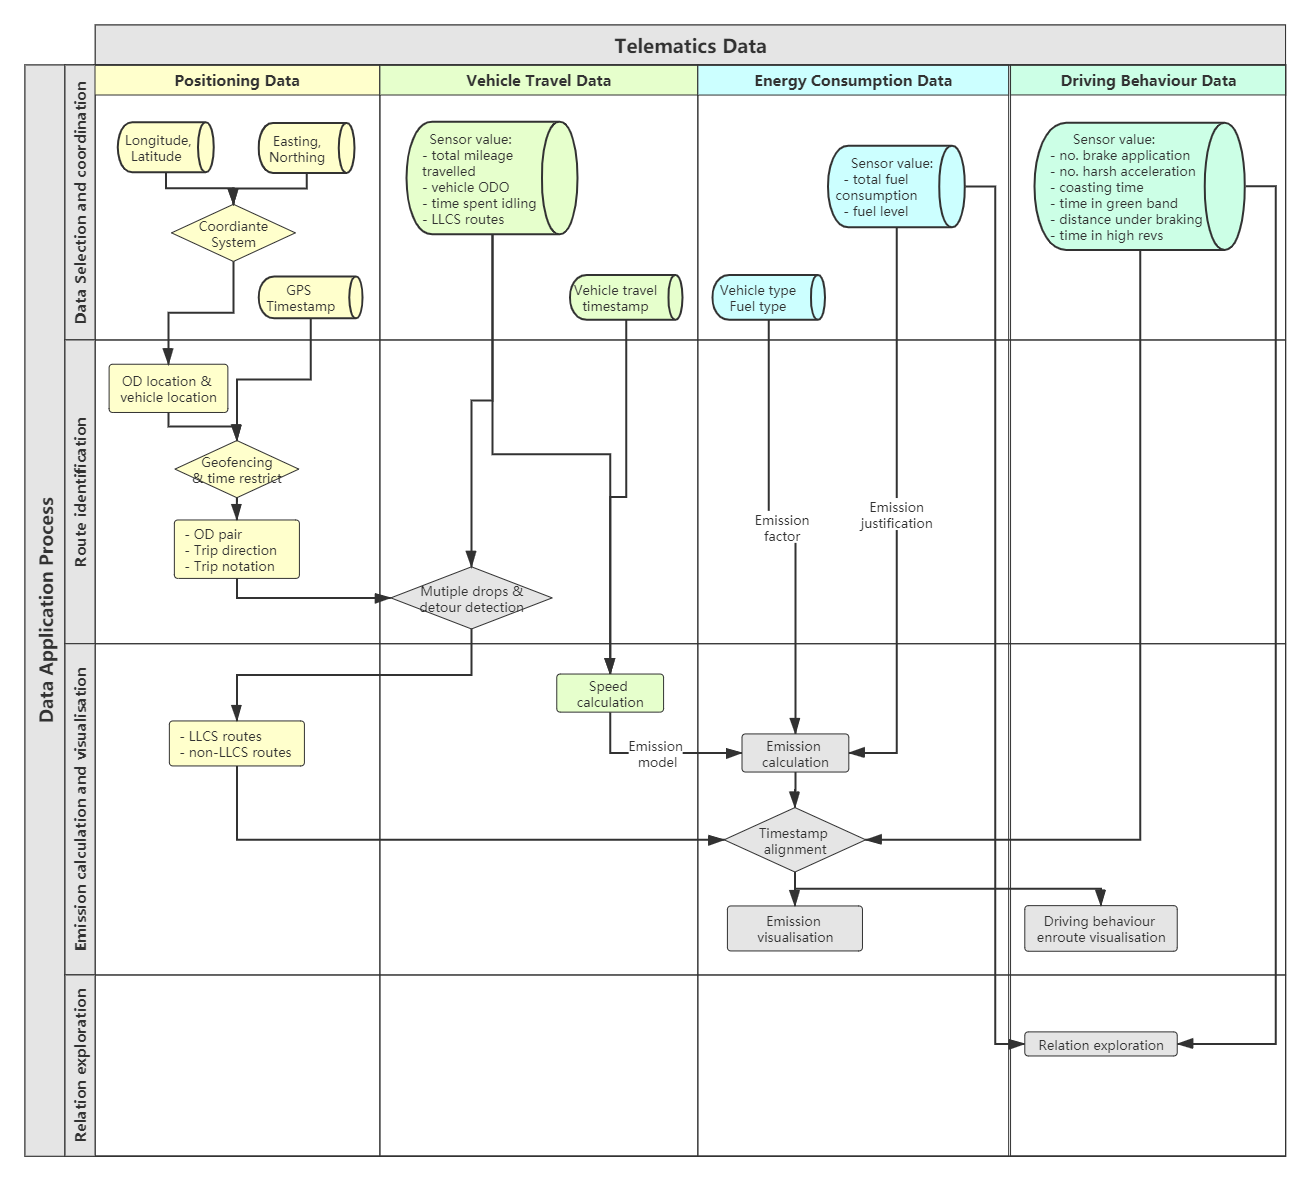
\includegraphics[width=1\textwidth]{LLCS telematics data utilisation framework.png} %插入图片,[]中设置图片大小,{}中是图片文件名
\caption{Framework of telematics data application} %最终文档中希望显示的图片标题
\label{Fig1} %用于文内引用的标签
\end{figure}


\section{Steps to extract routes information from telematics data}

\begin{figure}[H] %H为当前位置,!htb为忽略美学标准,htbp为浮动图形
\centering %图片居中
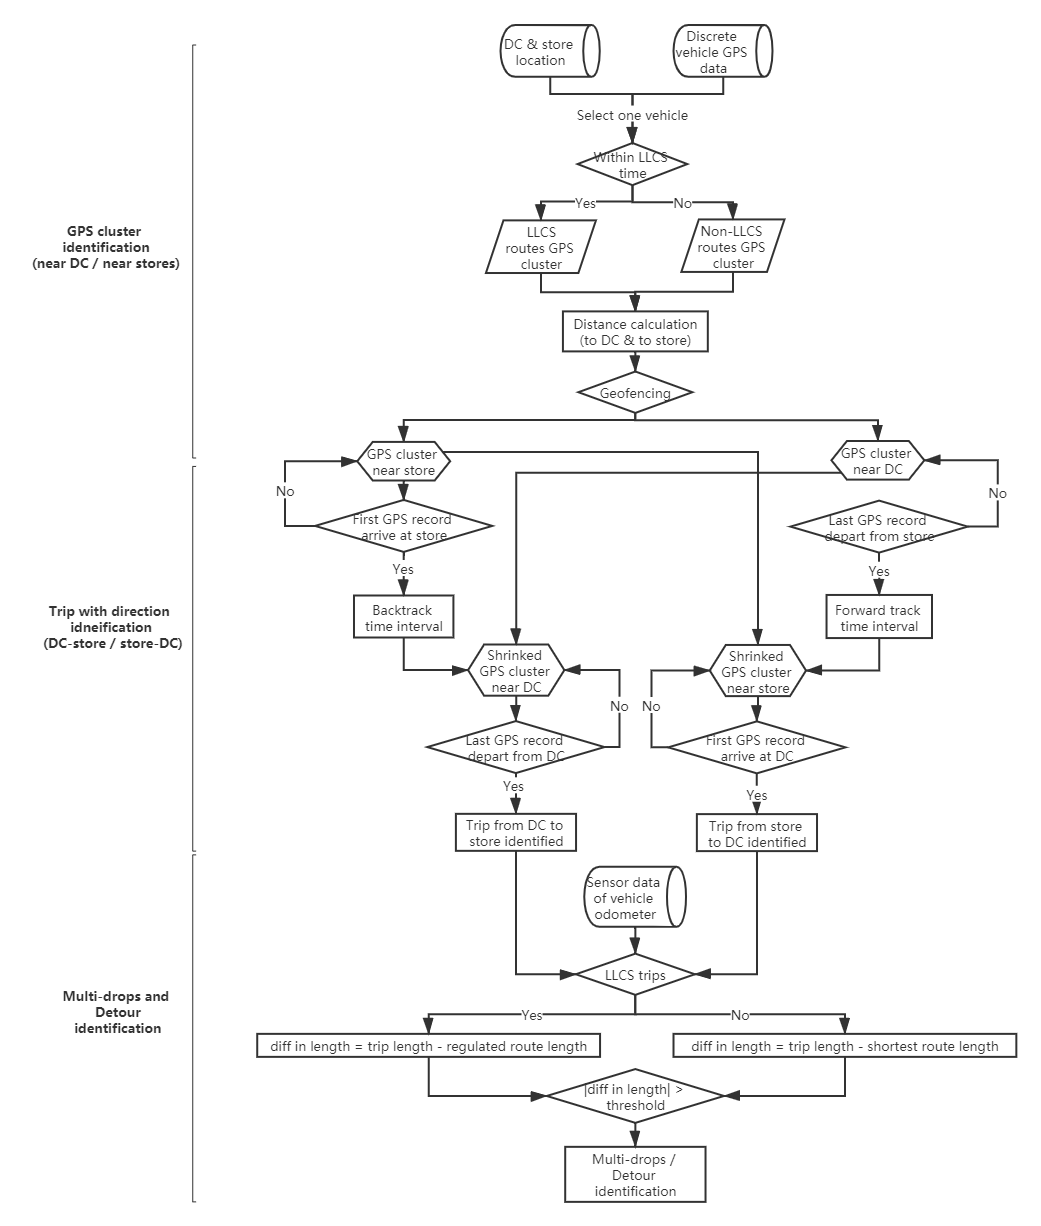
\includegraphics[width=1\textwidth]{OD pair identification.png} %插入图片,[]中设置图片大小,{}中是图片文件名
\caption{Steps to extract routes information from telematics data} %最终文档中希望显示的图片标题
\label{Fig1} %用于文内引用的标签
\end{figure}




\clearpage
\bibliographystyle{IEEEtranN}
\bibliography{llcsori} % if more than one, comma separated


\end{document}